\chapter{Semi-Leptonic Single Higgs Analytic Fits}
\label{sec:SLFits}

% \subsection{Continuum Background}
% \label{sec:SLBkgFits}

% The Semi-Leptonic DNN category ftests and fits to the data side bands to model the continuum background are shown below:

% \newpage 

% \begin{figure}[h!]
%     \setcounter{subfigure}{0}
%     \centering
%     \subfloat[fTest]{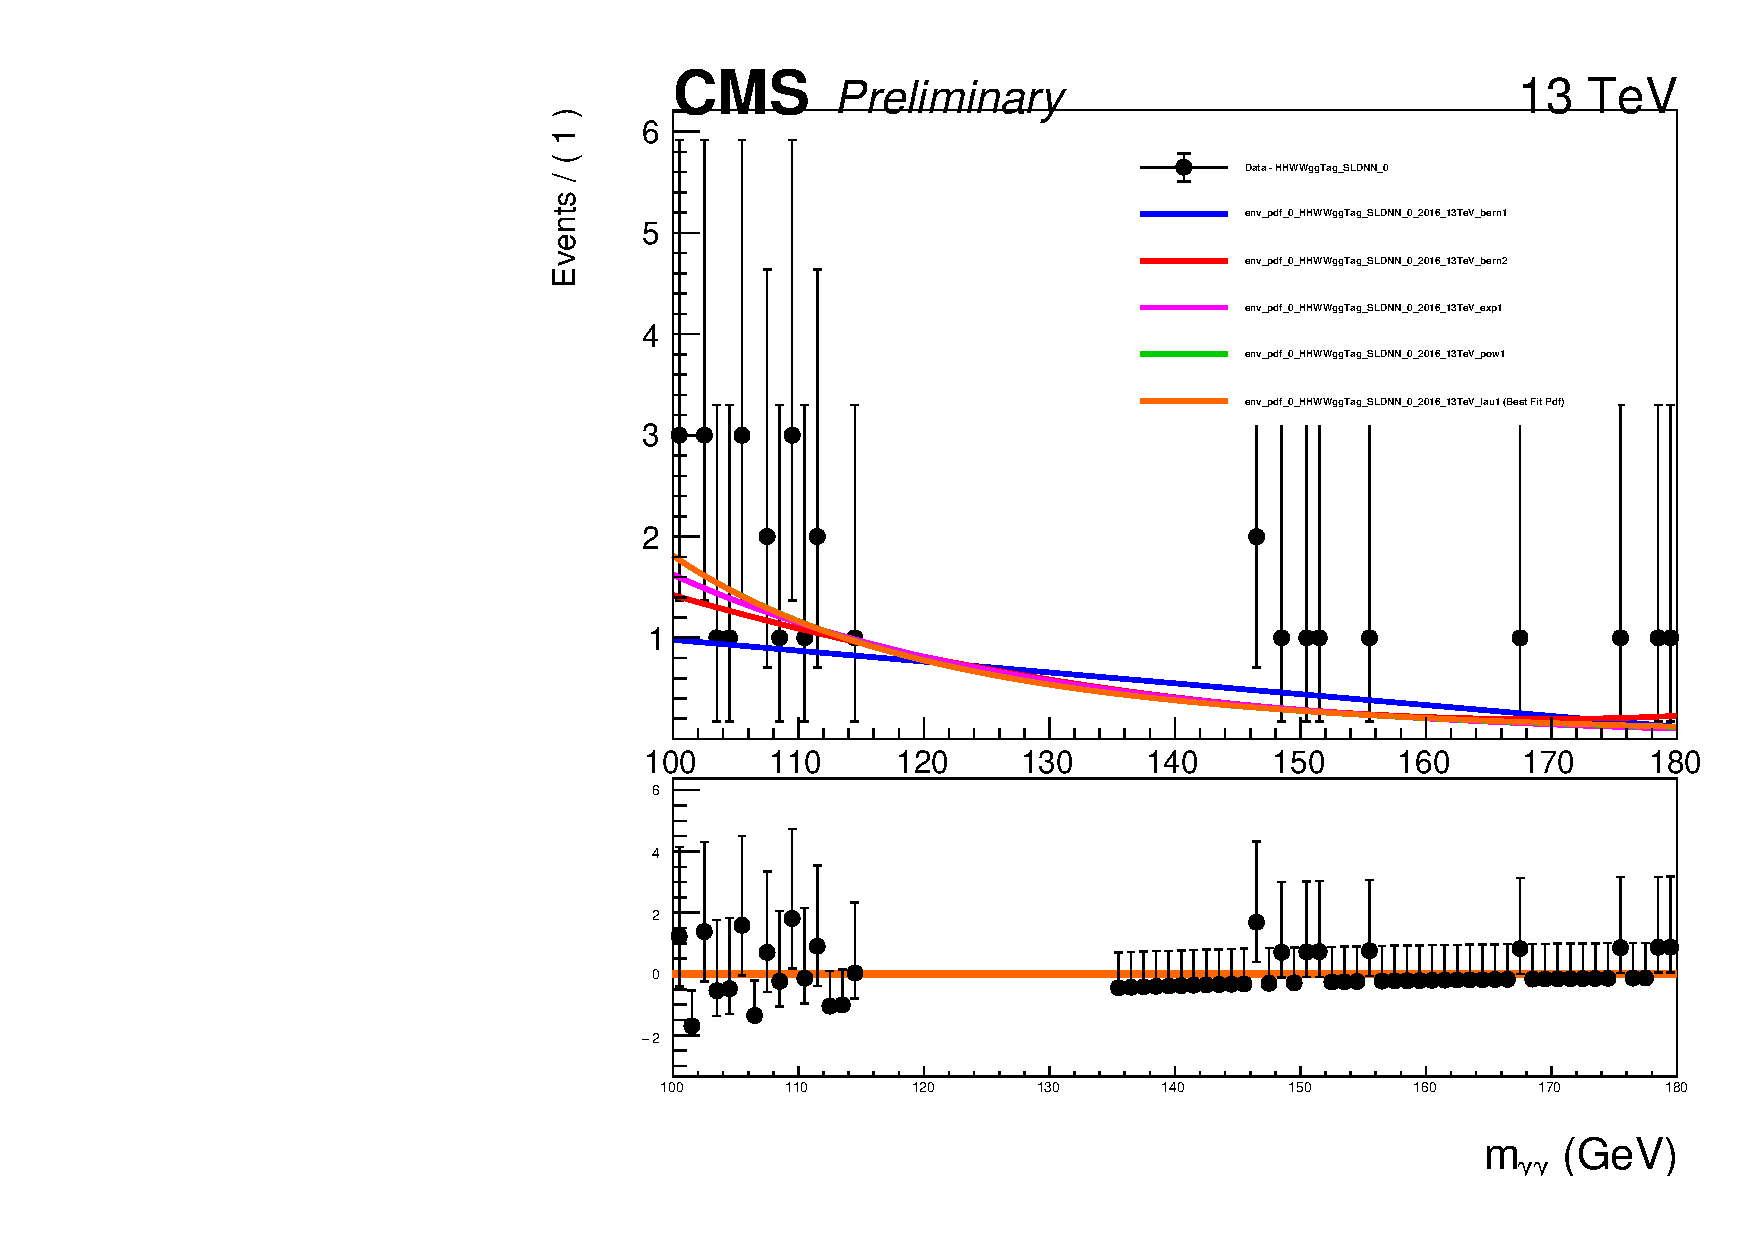
\includegraphics[width=0.45\textwidth]{Sections/HHWWgg/images/AnalyticFitting/ContinuumBackground/SL/2016/multipdf_HHWWggTag_SLDNN_0.pdf}}
%     \qquad
%     \subfloat[Background Fit]{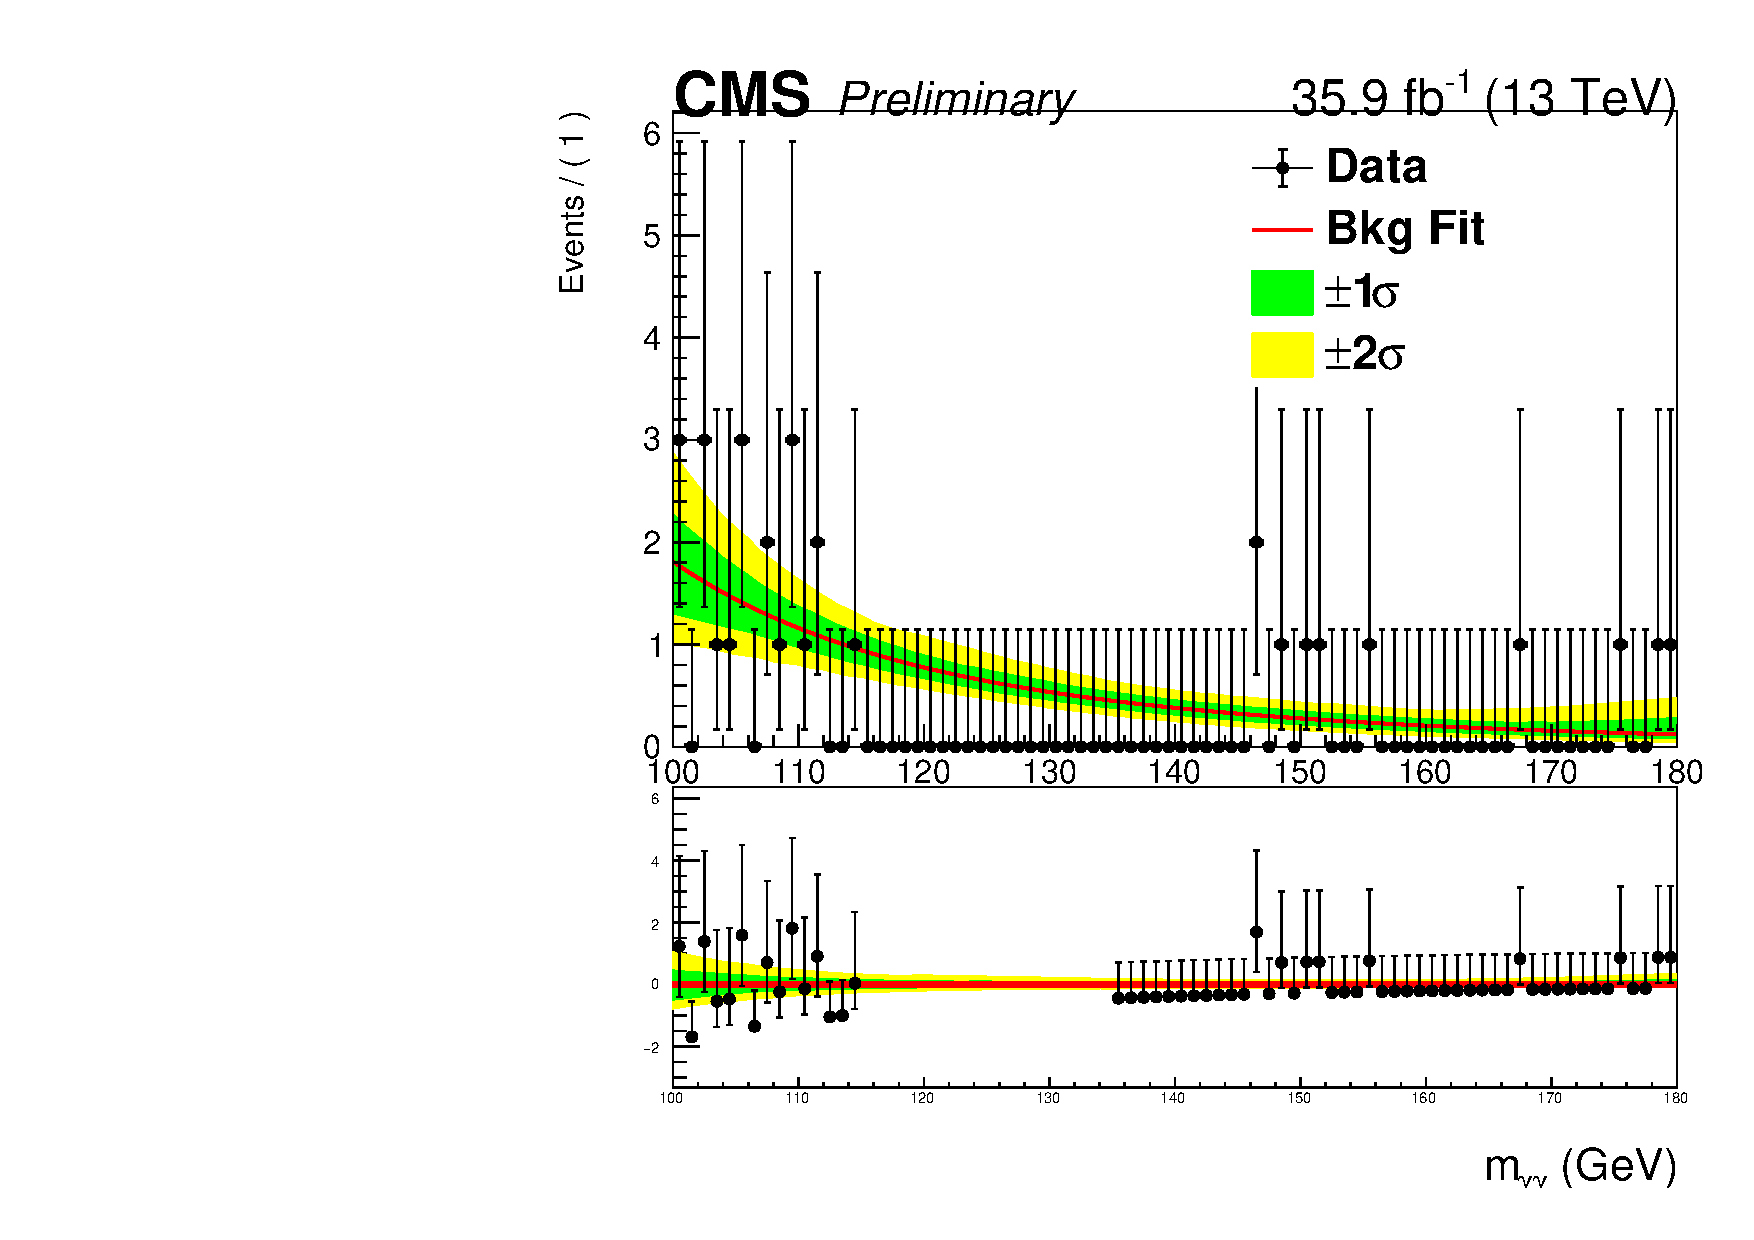
\includegraphics[width=0.45\textwidth]{Sections/HHWWgg/images/AnalyticFitting/ContinuumBackground/SL/2016/bkgplot_HHWWggTag_SLDNN_0.pdf}}
%     \caption{2016 Semi-Leptonic DNN Category 0 Background Model}
% \end{figure}

% \begin{figure}[h!]
%     \setcounter{subfigure}{0}
%     \centering
%     \subfloat[fTest]{\includegraphics[width=0.45\textwidth]{Sections/HHWWgg/images/AnalyticFitting/ContinuumBackground/SL/2017/multipdf_HHWWggTag_SLDNN_0.pdf}}
%     \qquad
%     \subfloat[Background Fit]{\includegraphics[width=0.45\textwidth]{Sections/HHWWgg/images/AnalyticFitting/ContinuumBackground/SL/2017/bkgplot_HHWWggTag_SLDNN_0.pdf}}
%     \caption{2017 Semi-Leptonic DNN Category 0 Background Model}
% \end{figure}

% \newpage 

% \begin{figure}[h!]
%     \setcounter{subfigure}{0}
%     \centering
%     \subfloat[fTest]{\includegraphics[width=0.45\textwidth]{Sections/HHWWgg/images/AnalyticFitting/ContinuumBackground/SL/2018/multipdf_HHWWggTag_SLDNN_0.pdf}}
%     \qquad
%     \subfloat[Background Fit]{\includegraphics[width=0.45\textwidth]{Sections/HHWWgg/images/AnalyticFitting/ContinuumBackground/SL/2018/bkgplot_HHWWggTag_SLDNN_0.pdf}}
%     \caption{2018 Semi-Leptonic DNN Category 0 Background Model}
% \end{figure}

% \begin{figure}[h!]
%     \setcounter{subfigure}{0}
%     \centering
%     \subfloat[fTest]{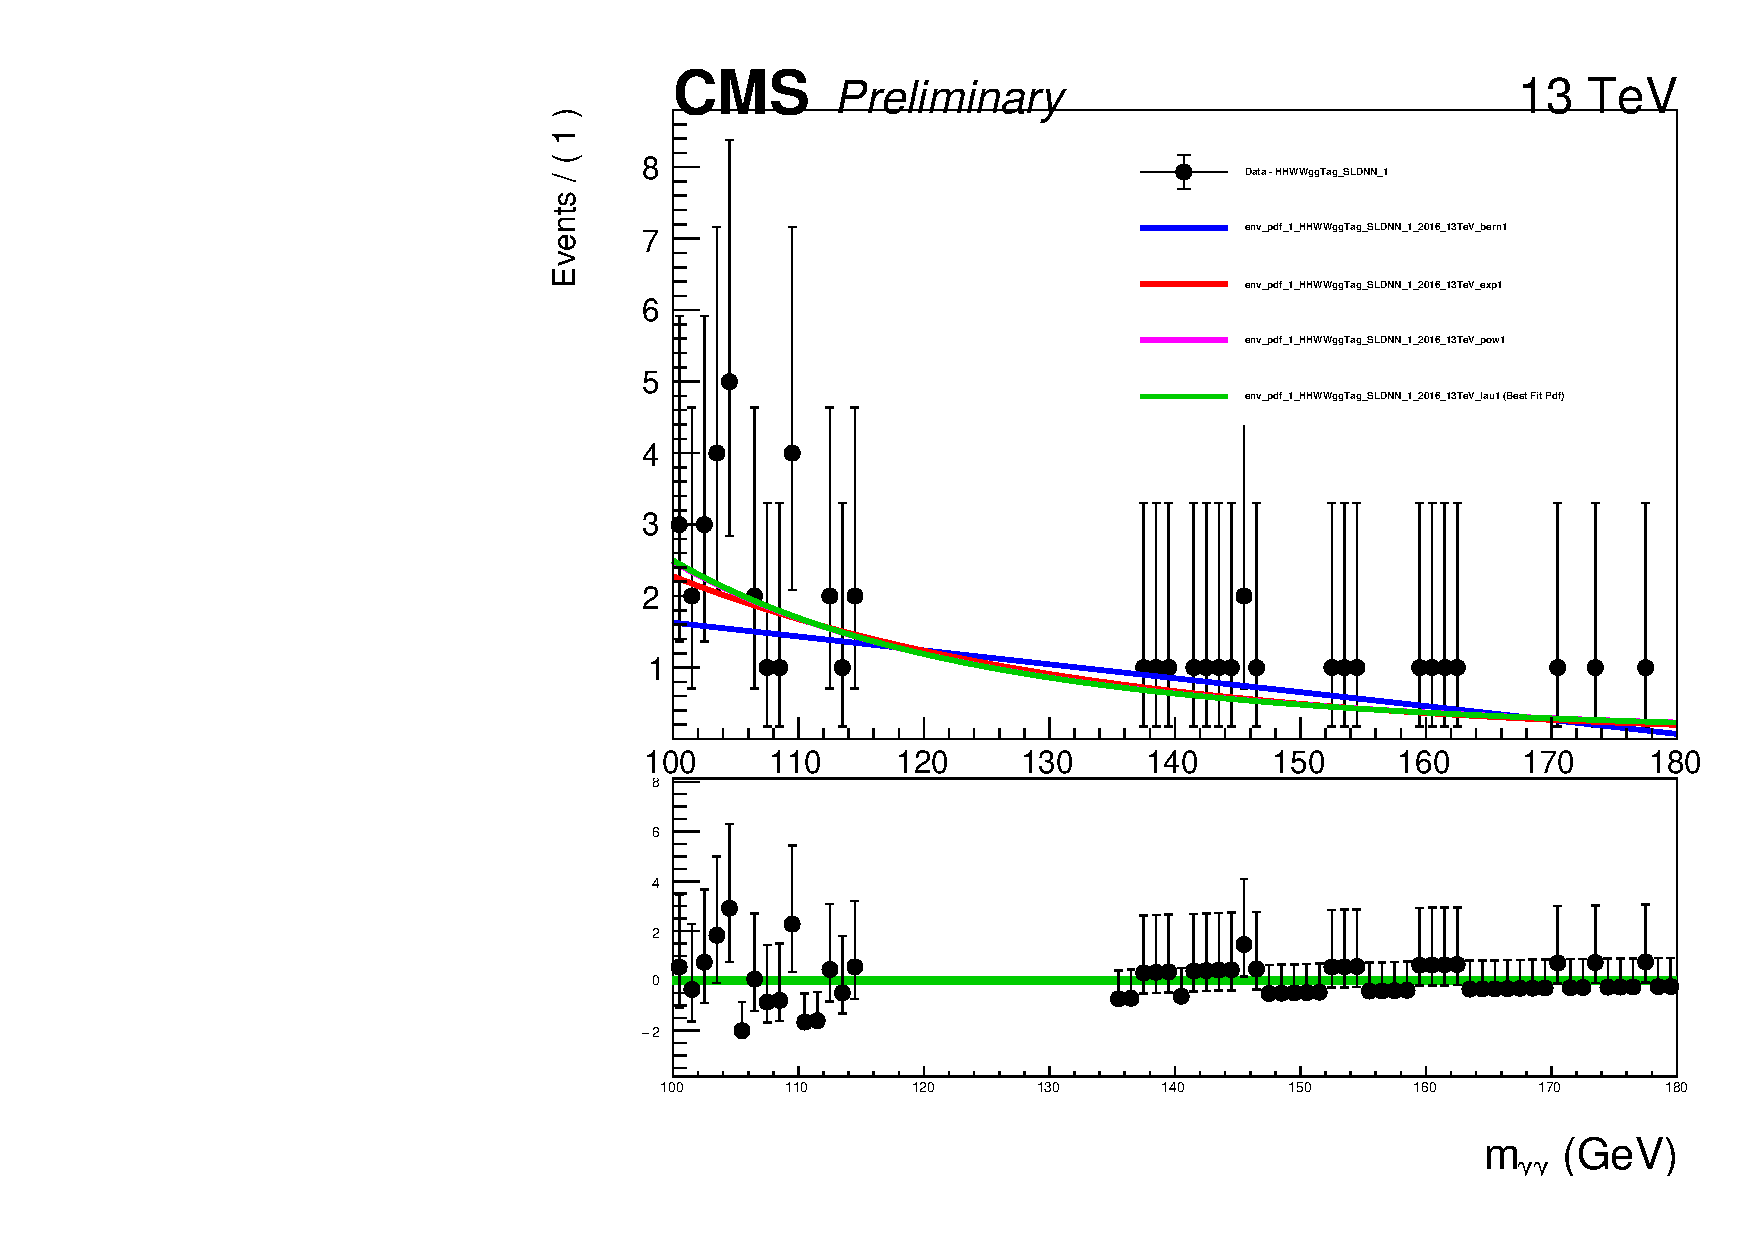
\includegraphics[width=0.45\textwidth]{Sections/HHWWgg/images/AnalyticFitting/ContinuumBackground/SL/2016/multipdf_HHWWggTag_SLDNN_1.pdf}}
%     \qquad
%     \subfloat[Background Fit]{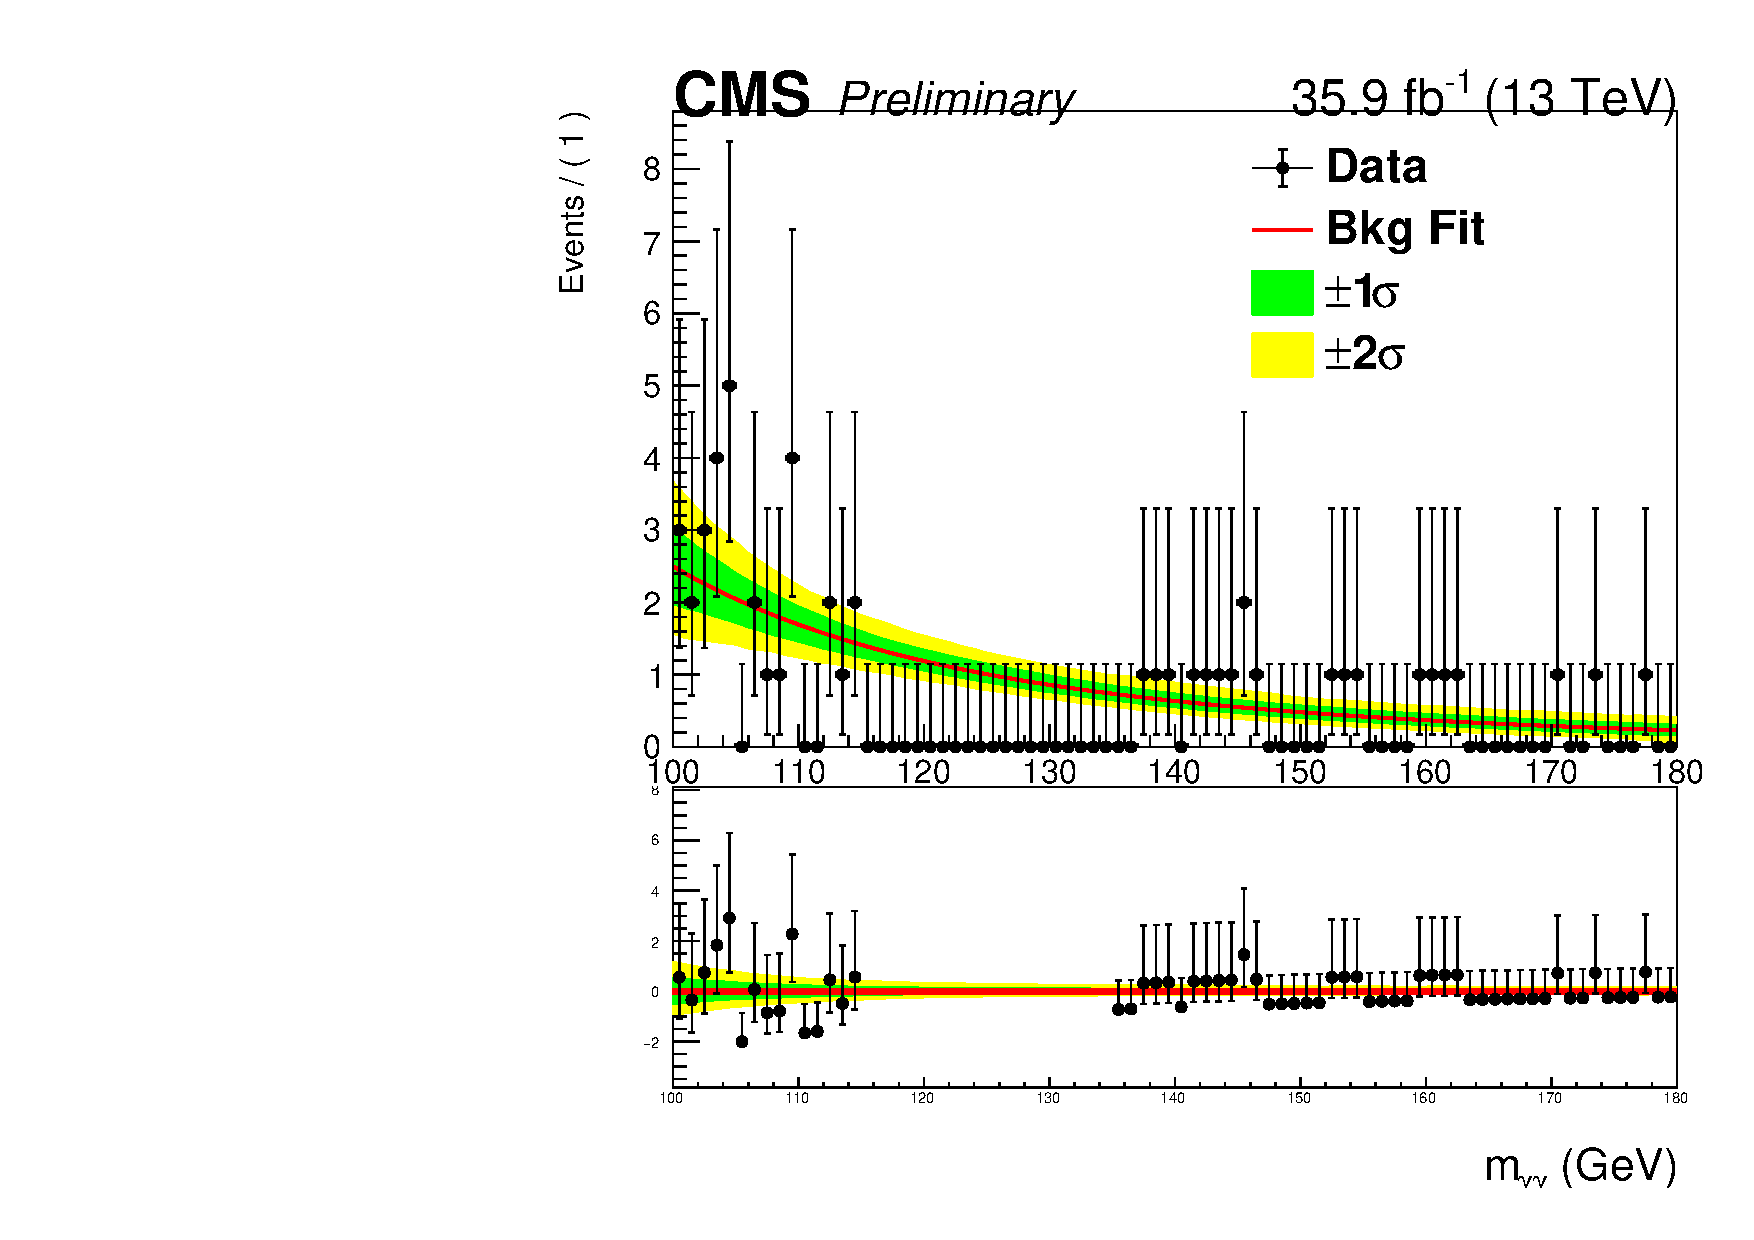
\includegraphics[width=0.45\textwidth]{Sections/HHWWgg/images/AnalyticFitting/ContinuumBackground/SL/2016/bkgplot_HHWWggTag_SLDNN_1.pdf}}
%     \caption{2016 Semi-Leptonic DNN Category 1 Background Model}
% \end{figure}

% \newpage 

% \begin{figure}[h!]
%     \setcounter{subfigure}{0}
%     \centering
%     \subfloat[fTest]{\includegraphics[width=0.45\textwidth]{Sections/HHWWgg/images/AnalyticFitting/ContinuumBackground/SL/2017/multipdf_HHWWggTag_SLDNN_1.pdf}}
%     \qquad
%     \subfloat[Background Fit]{\includegraphics[width=0.45\textwidth]{Sections/HHWWgg/images/AnalyticFitting/ContinuumBackground/SL/2017/bkgplot_HHWWggTag_SLDNN_1.pdf}}
%     \caption{2017 Semi-Leptonic DNN Category 1 Background Model}
% \end{figure}

% \begin{figure}[h!]
%     \setcounter{subfigure}{0}
%     \centering
%     \subfloat[fTest]{\includegraphics[width=0.45\textwidth]{Sections/HHWWgg/images/AnalyticFitting/ContinuumBackground/SL/2018/multipdf_HHWWggTag_SLDNN_1.pdf}}
%     \qquad
%     \subfloat[Background Fit]{\includegraphics[width=0.45\textwidth]{Sections/HHWWgg/images/AnalyticFitting/ContinuumBackground/SL/2018/bkgplot_HHWWggTag_SLDNN_1.pdf}}
%     \caption{2018 Semi-Leptonic DNN Category 1 Background Model}
% \end{figure}

% \newpage 

% \begin{figure}[h!]
%     \setcounter{subfigure}{0}
%     \centering
%     \subfloat[fTest]{\includegraphics[width=0.45\textwidth]{Sections/HHWWgg/images/AnalyticFitting/ContinuumBackground/SL/2016/multipdf_HHWWggTag_SLDNN_2.pdf}}
%     \qquad
%     \subfloat[Background Fit]{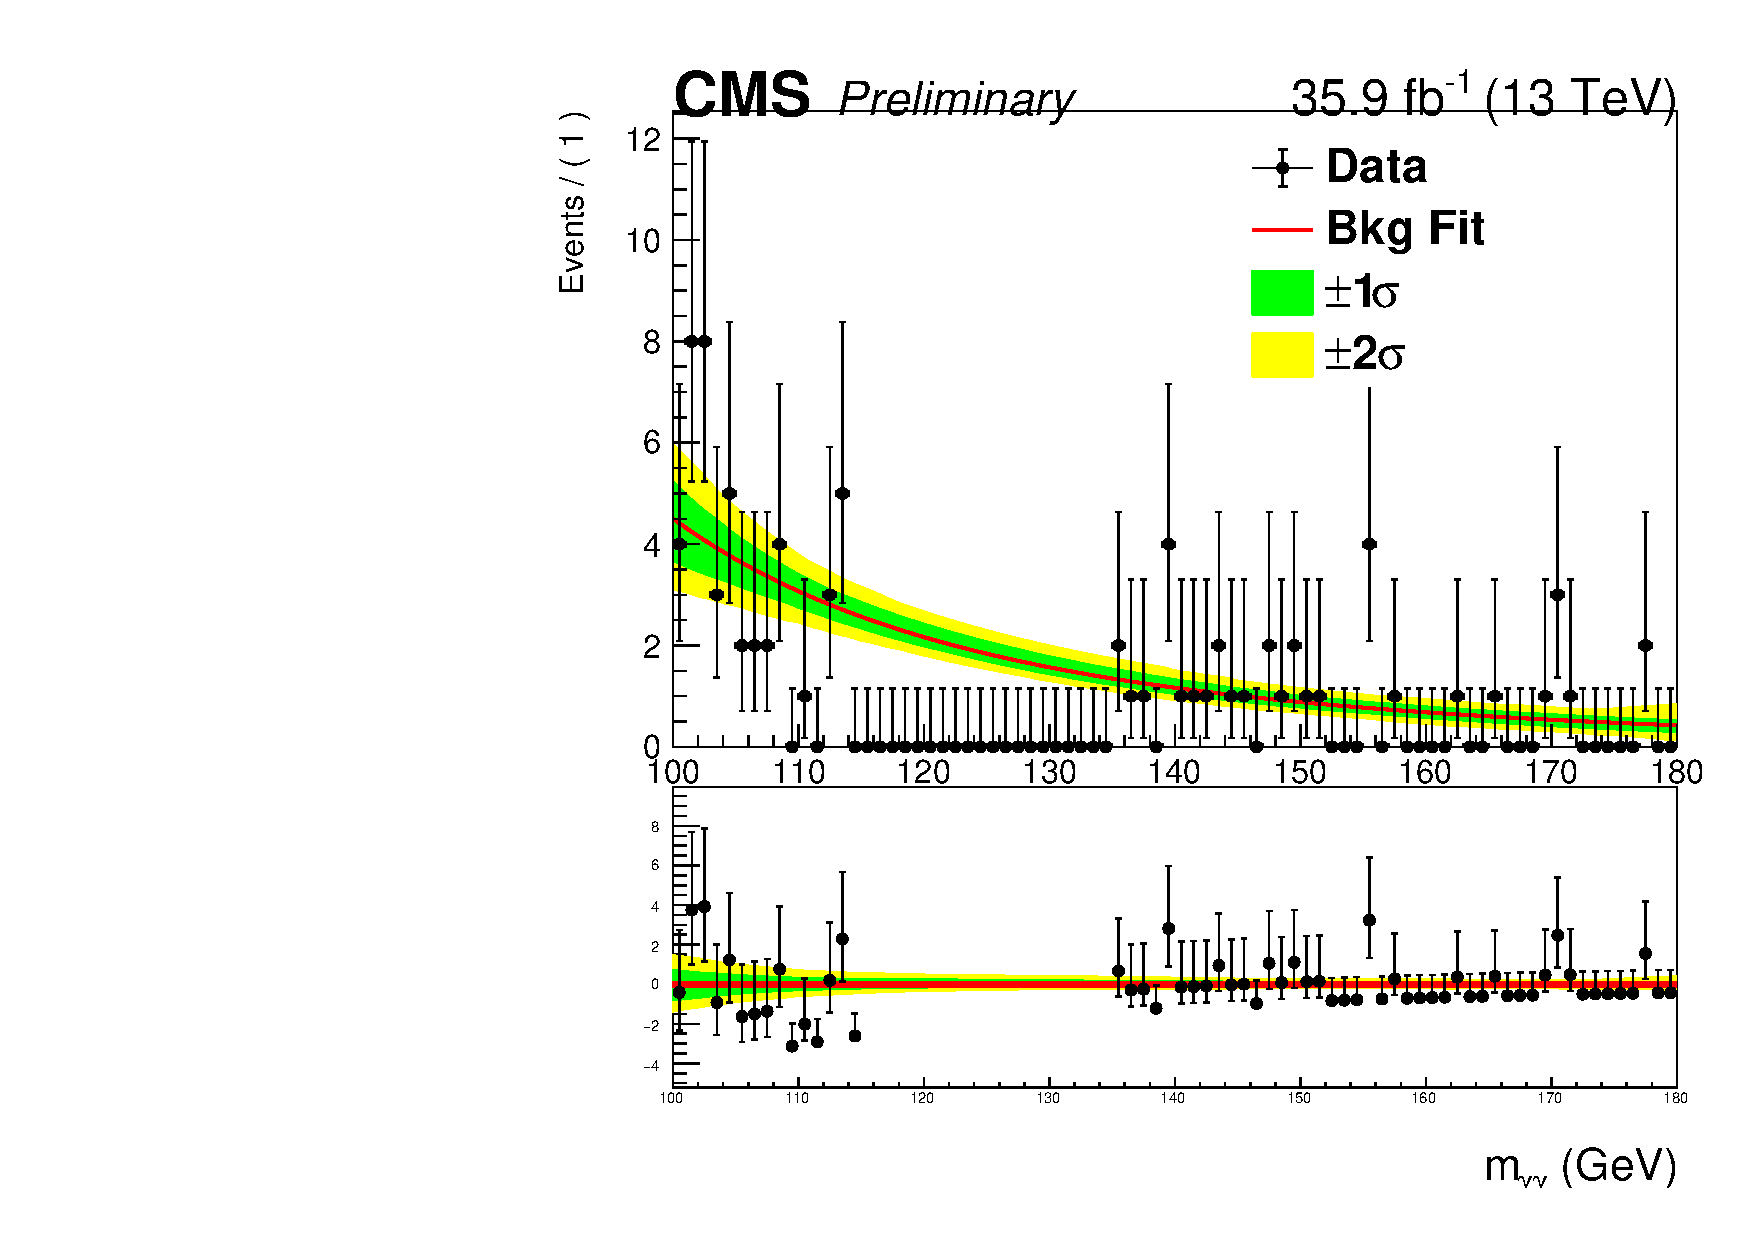
\includegraphics[width=0.45\textwidth]{Sections/HHWWgg/images/AnalyticFitting/ContinuumBackground/SL/2016/bkgplot_HHWWggTag_SLDNN_2.pdf}}
%     \caption{2016 Semi-Leptonic DNN Category 2 Background Model}
% \end{figure}

% \begin{figure}[h!]
%     \setcounter{subfigure}{0}
%     \centering
%     \subfloat[fTest]{\includegraphics[width=0.45\textwidth]{Sections/HHWWgg/images/AnalyticFitting/ContinuumBackground/SL/2017/multipdf_HHWWggTag_SLDNN_2.pdf}}
%     \qquad
%     \subfloat[Background Fit]{\includegraphics[width=0.45\textwidth]{Sections/HHWWgg/images/AnalyticFitting/ContinuumBackground/SL/2017/bkgplot_HHWWggTag_SLDNN_2.pdf}}
%     \caption{2017 Semi-Leptonic DNN Category 2 Background Model}
% \end{figure}

% \newpage 

% \begin{figure}[h!]
%     \setcounter{subfigure}{0}
%     \centering
%     \subfloat[fTest]{\includegraphics[width=0.45\textwidth]{Sections/HHWWgg/images/AnalyticFitting/ContinuumBackground/SL/2018/multipdf_HHWWggTag_SLDNN_2.pdf}}
%     \qquad
%     \subfloat[Background Fit]{\includegraphics[width=0.45\textwidth]{Sections/HHWWgg/images/AnalyticFitting/ContinuumBackground/SL/2018/bkgplot_HHWWggTag_SLDNN_2.pdf}}
%     \caption{2018 Semi-Leptonic DNN Category 2 Background Model}
% \end{figure}

% \begin{figure}[h!]
%     \setcounter{subfigure}{0}
%     \centering
%     \subfloat[fTest]{\includegraphics[width=0.45\textwidth]{Sections/HHWWgg/images/AnalyticFitting/ContinuumBackground/SL/2016/multipdf_HHWWggTag_SLDNN_3.pdf}}
%     \qquad
%     \subfloat[Background Fit]{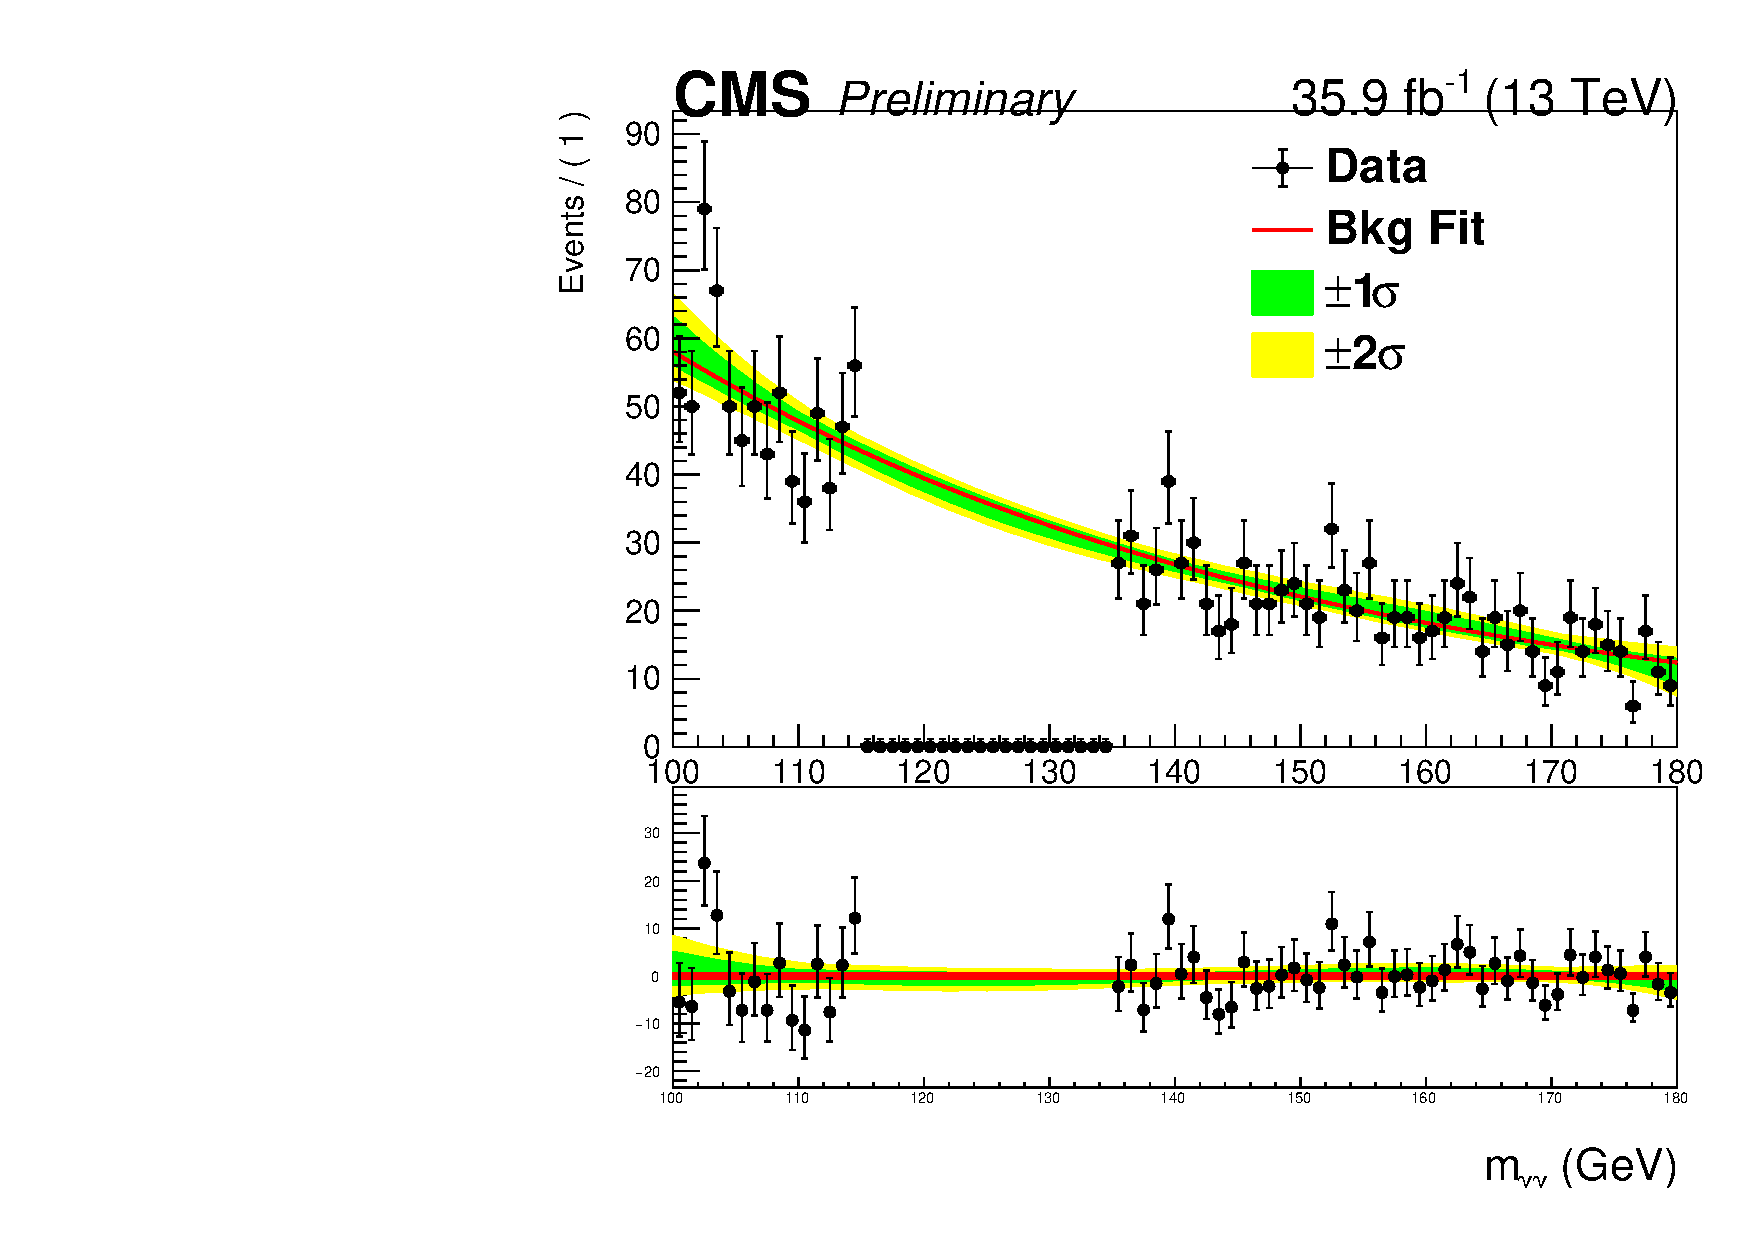
\includegraphics[width=0.45\textwidth]{Sections/HHWWgg/images/AnalyticFitting/ContinuumBackground/SL/2016/bkgplot_HHWWggTag_SLDNN_3.pdf}}
%     \caption{2016 Semi-Leptonic DNN Category 3 Background Model}
% \end{figure}

% \newpage 

% \begin{figure}[h!]
%     \setcounter{subfigure}{0}
%     \centering
%     \subfloat[fTest]{\includegraphics[width=0.45\textwidth]{Sections/HHWWgg/images/AnalyticFitting/ContinuumBackground/SL/2017/multipdf_HHWWggTag_SLDNN_3.pdf}}
%     \qquad
%     \subfloat[Background Fit]{\includegraphics[width=0.45\textwidth]{Sections/HHWWgg/images/AnalyticFitting/ContinuumBackground/SL/2017/bkgplot_HHWWggTag_SLDNN_3.pdf}}
%     \caption{2017 Semi-Leptonic DNN Category 3 Background Model}
% \end{figure}

% \begin{figure}[h!]
%     \setcounter{subfigure}{0}
%     \centering
%     \subfloat[fTest]{\includegraphics[width=0.45\textwidth]{Sections/HHWWgg/images/AnalyticFitting/ContinuumBackground/SL/2018/multipdf_HHWWggTag_SLDNN_3.pdf}}
%     \qquad
%     \subfloat[Background Fit]{\includegraphics[width=0.45\textwidth]{Sections/HHWWgg/images/AnalyticFitting/ContinuumBackground/SL/2018/bkgplot_HHWWggTag_SLDNN_3.pdf}}
%     \caption{2018 Semi-Leptonic DNN Category 3 Background Model}
% \end{figure}

\section{Single Higgs}
\label{sec:SLSingleHiggsFits}

The Semi-Leptonic DNN category fits to Single Higgs processes are shown below.

\newpage 

\begin{figure}[h!]
    \setcounter{subfigure}{0}
    \centering
    \subfloat[GluGluHToGG]{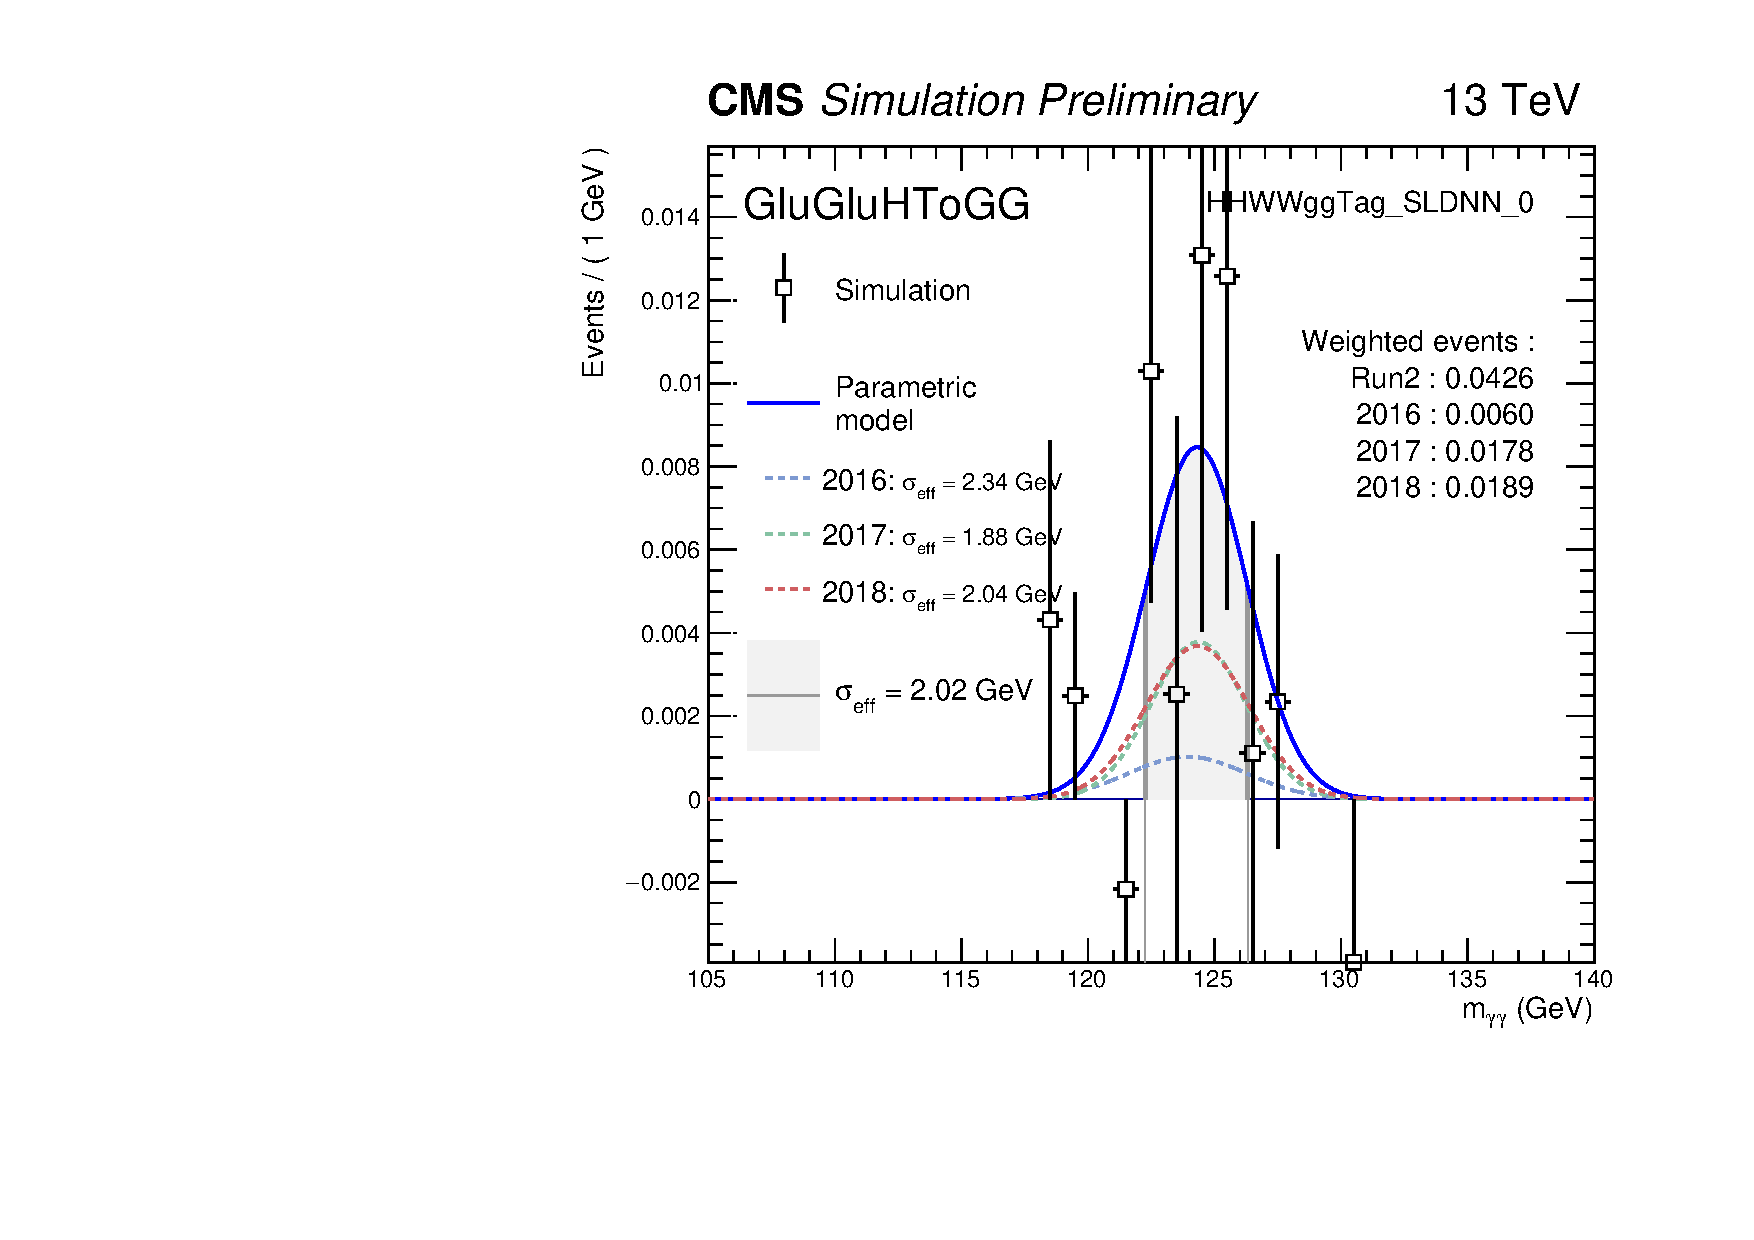
\includegraphics[width=0.45\textwidth]{Sections/HHWWgg/images/AnalyticFitting/SingleHiggs/ggH/SL/smodel_HHWWggTag_SLDNN_0.pdf}}
    \qquad
    \subfloat[VBFHToGG]{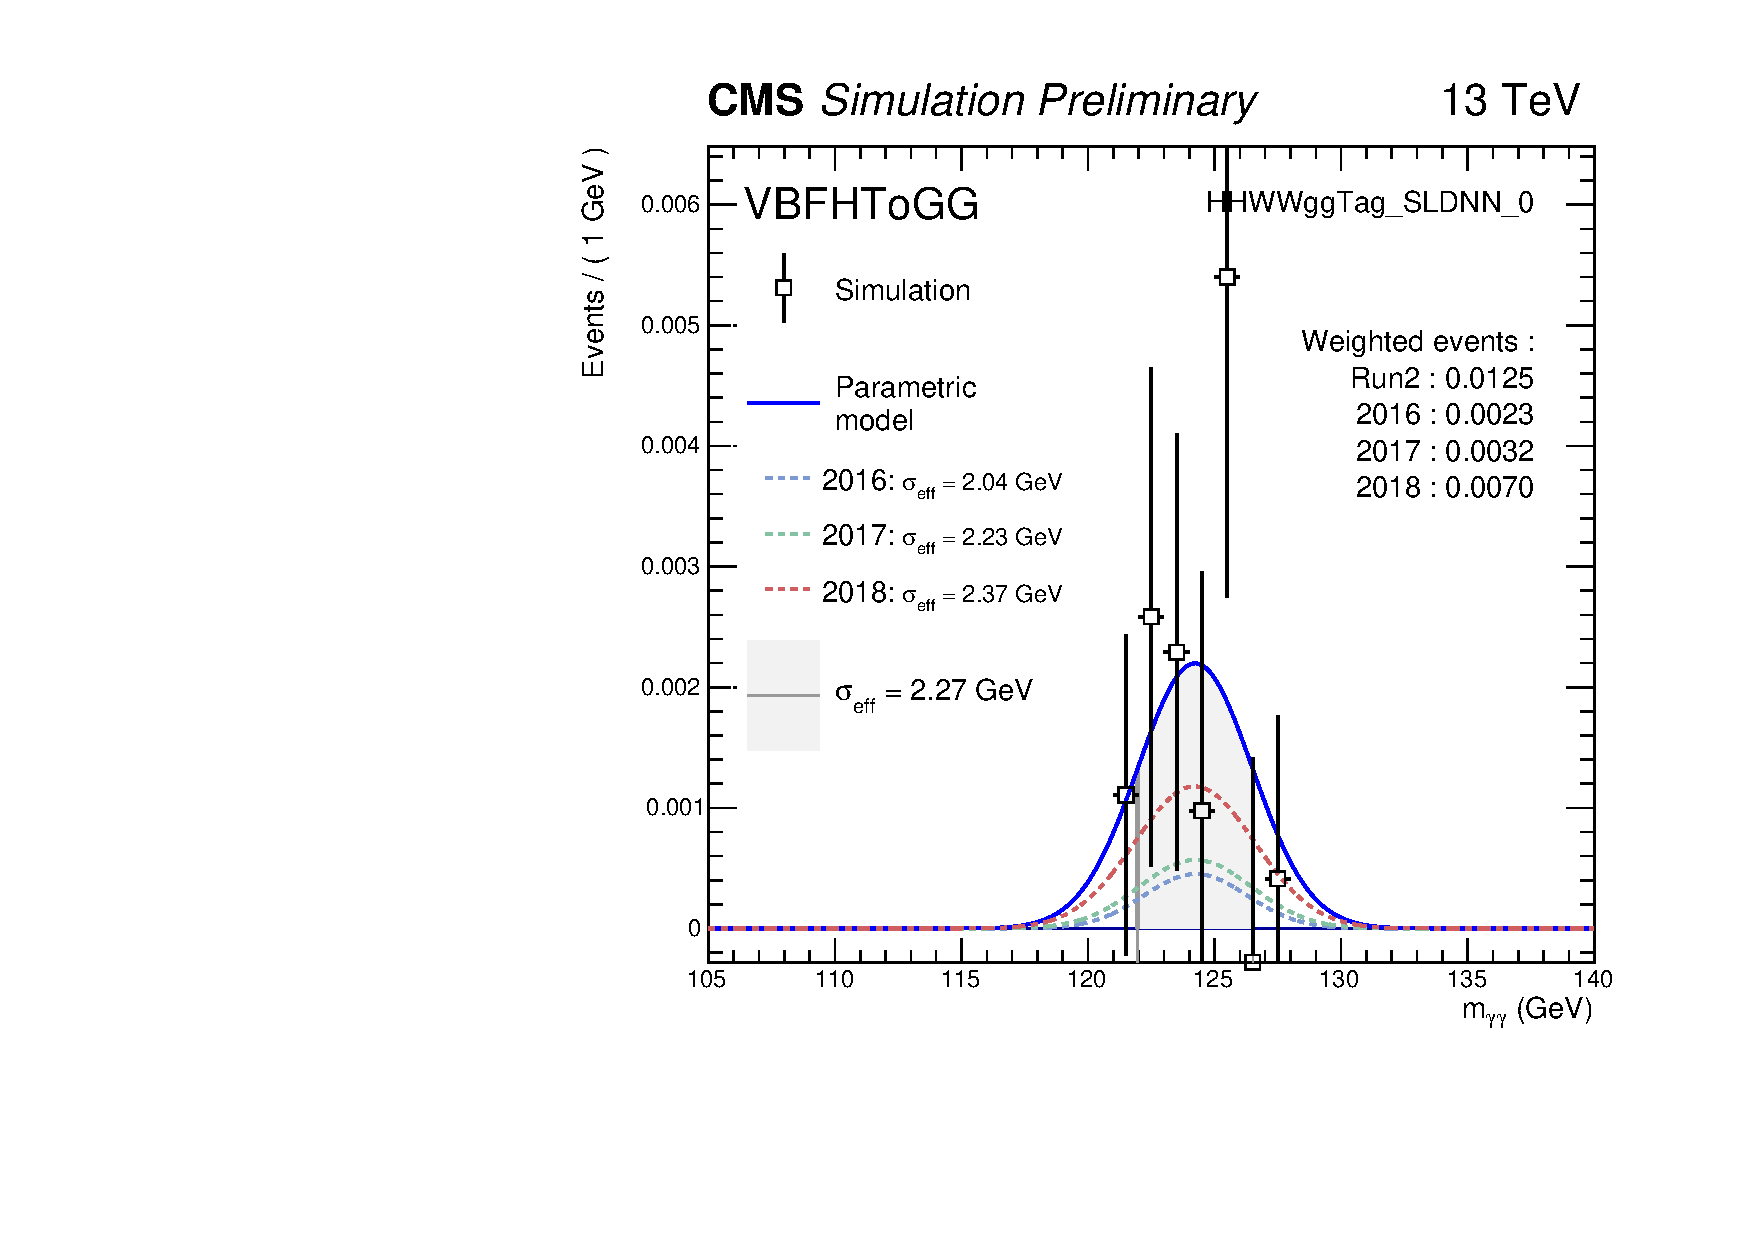
\includegraphics[width=0.45\textwidth]{Sections/HHWWgg/images/AnalyticFitting/SingleHiggs/VBFH/SL/smodel_HHWWggTag_SLDNN_0.pdf}}
    \caption{Semi-Leptonic DNN Category 0 Single Higgs Models}
\end{figure}

\begin{figure}[h!]
    \setcounter{subfigure}{0}
    \centering
    \subfloat[VHToGG]{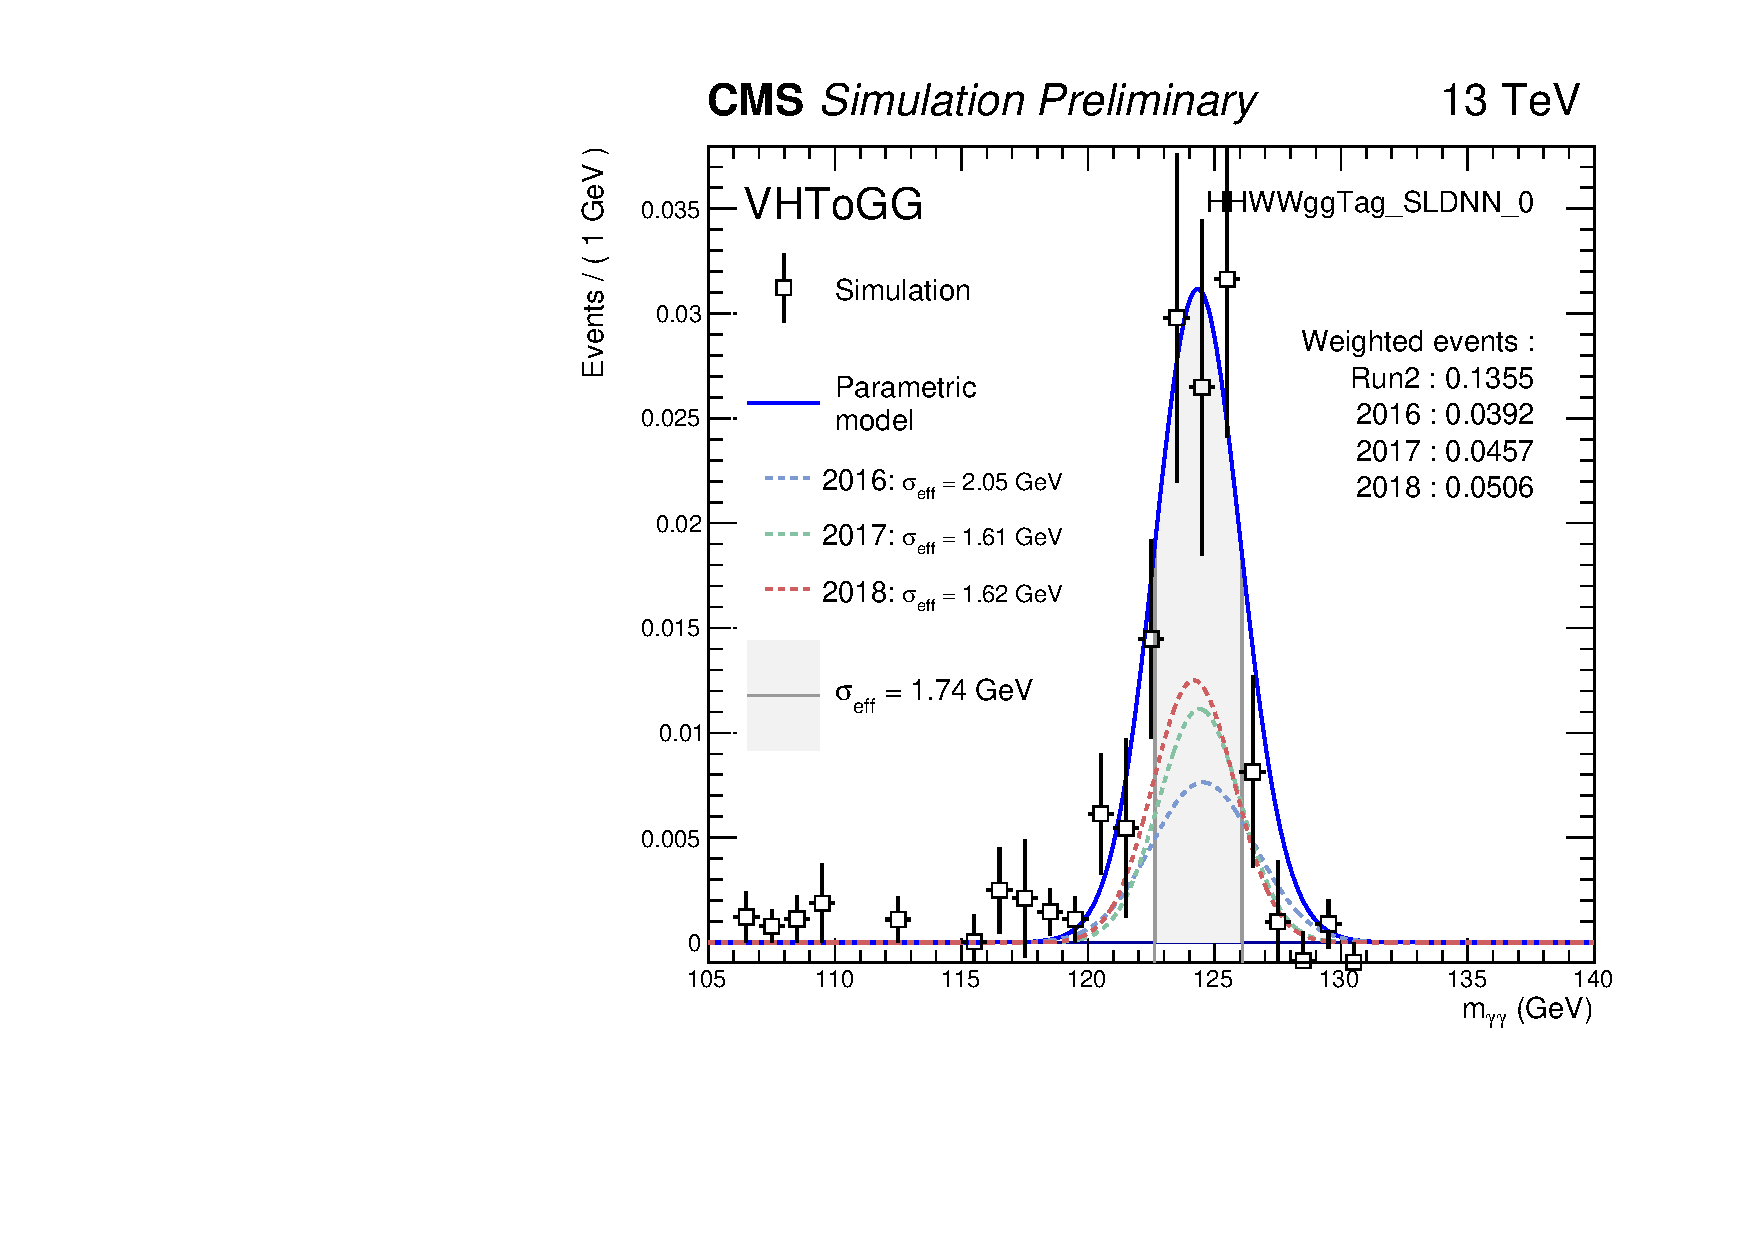
\includegraphics[width=0.45\textwidth]{Sections/HHWWgg/images/AnalyticFitting/SingleHiggs/VH/SL/smodel_HHWWggTag_SLDNN_0.pdf}}
    \qquad
    \subfloat[ttHJetToGG]{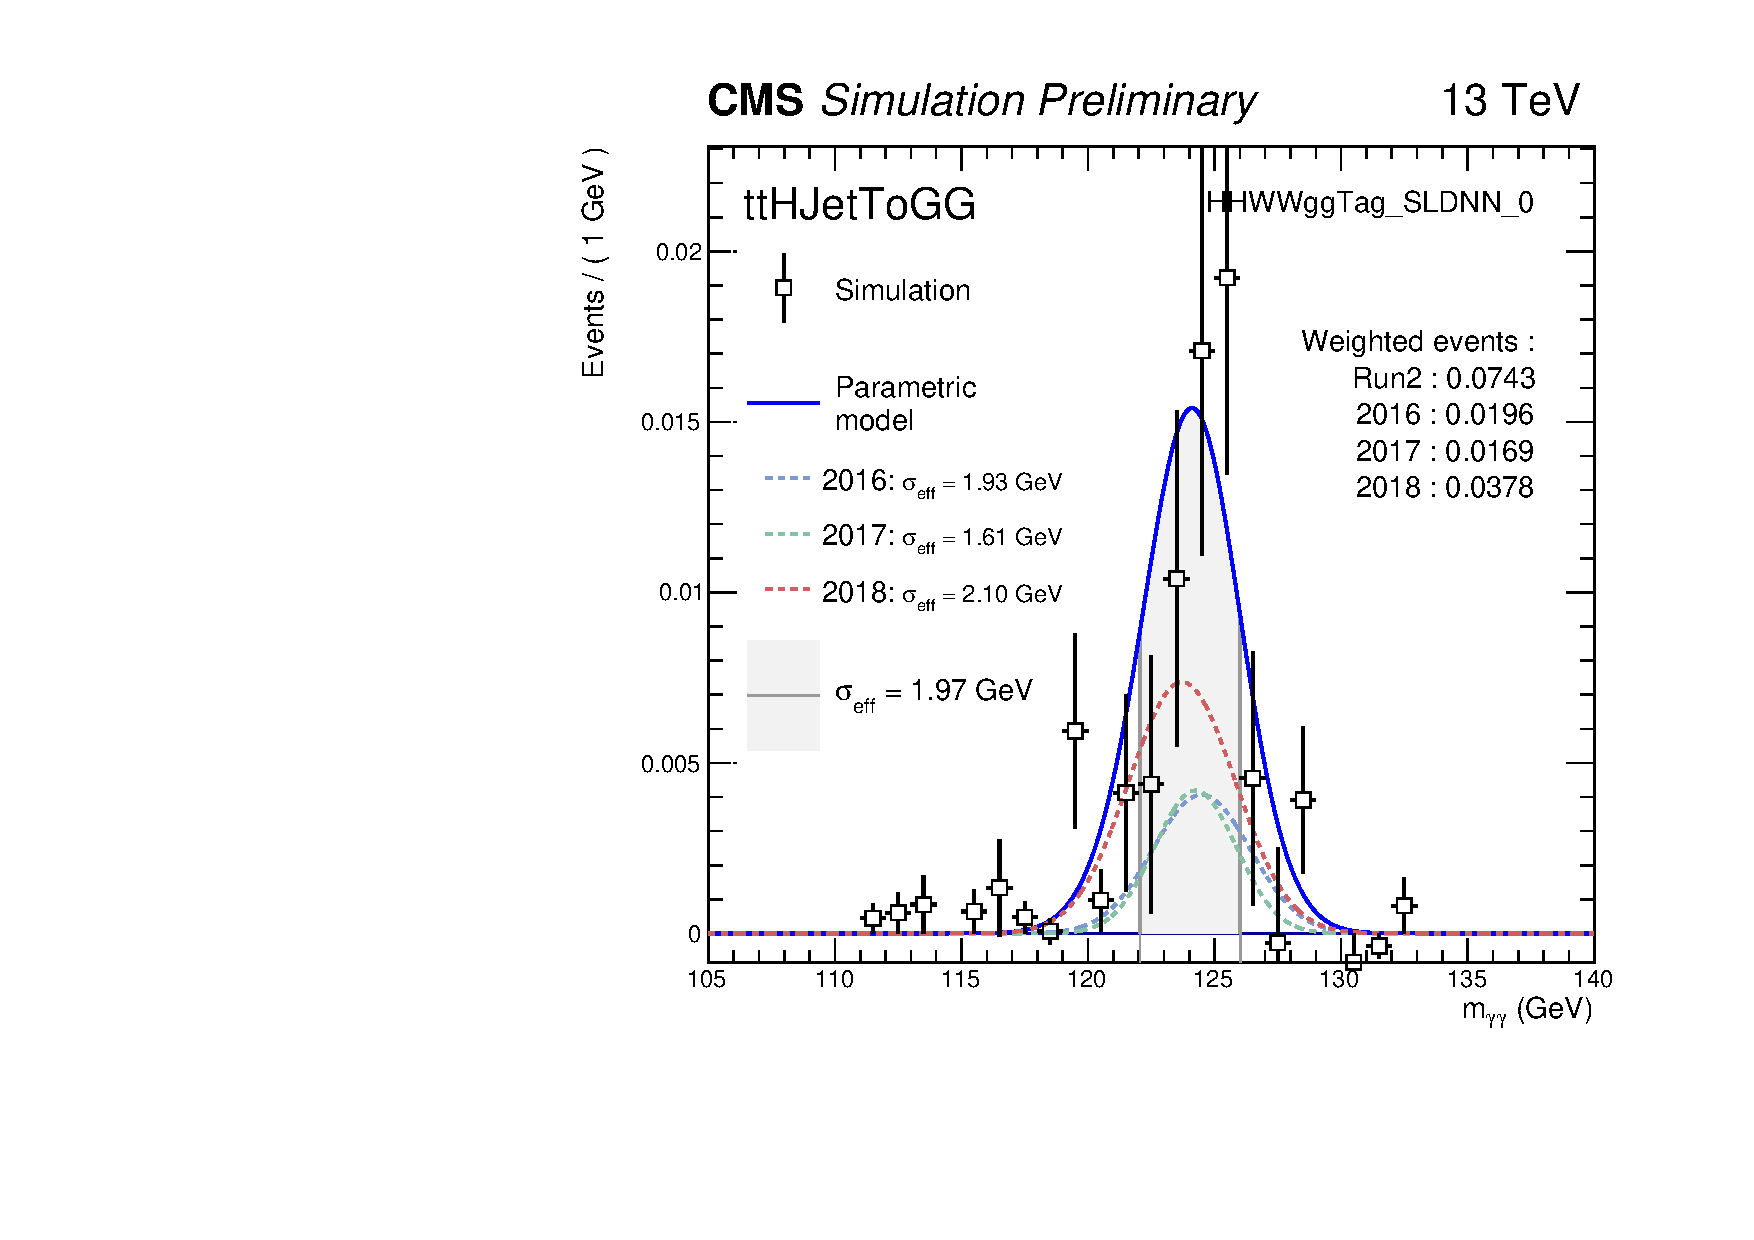
\includegraphics[width=0.45\textwidth]{Sections/HHWWgg/images/AnalyticFitting/SingleHiggs/ttHJet/SL/smodel_HHWWggTag_SLDNN_0.pdf}}
    \caption{Semi-Leptonic DNN Category 0 Single Higgs Models}
\end{figure}

\newpage 

\begin{figure}[h!]
    \setcounter{subfigure}{0}
    \centering
    \subfloat[GluGluHToGG]{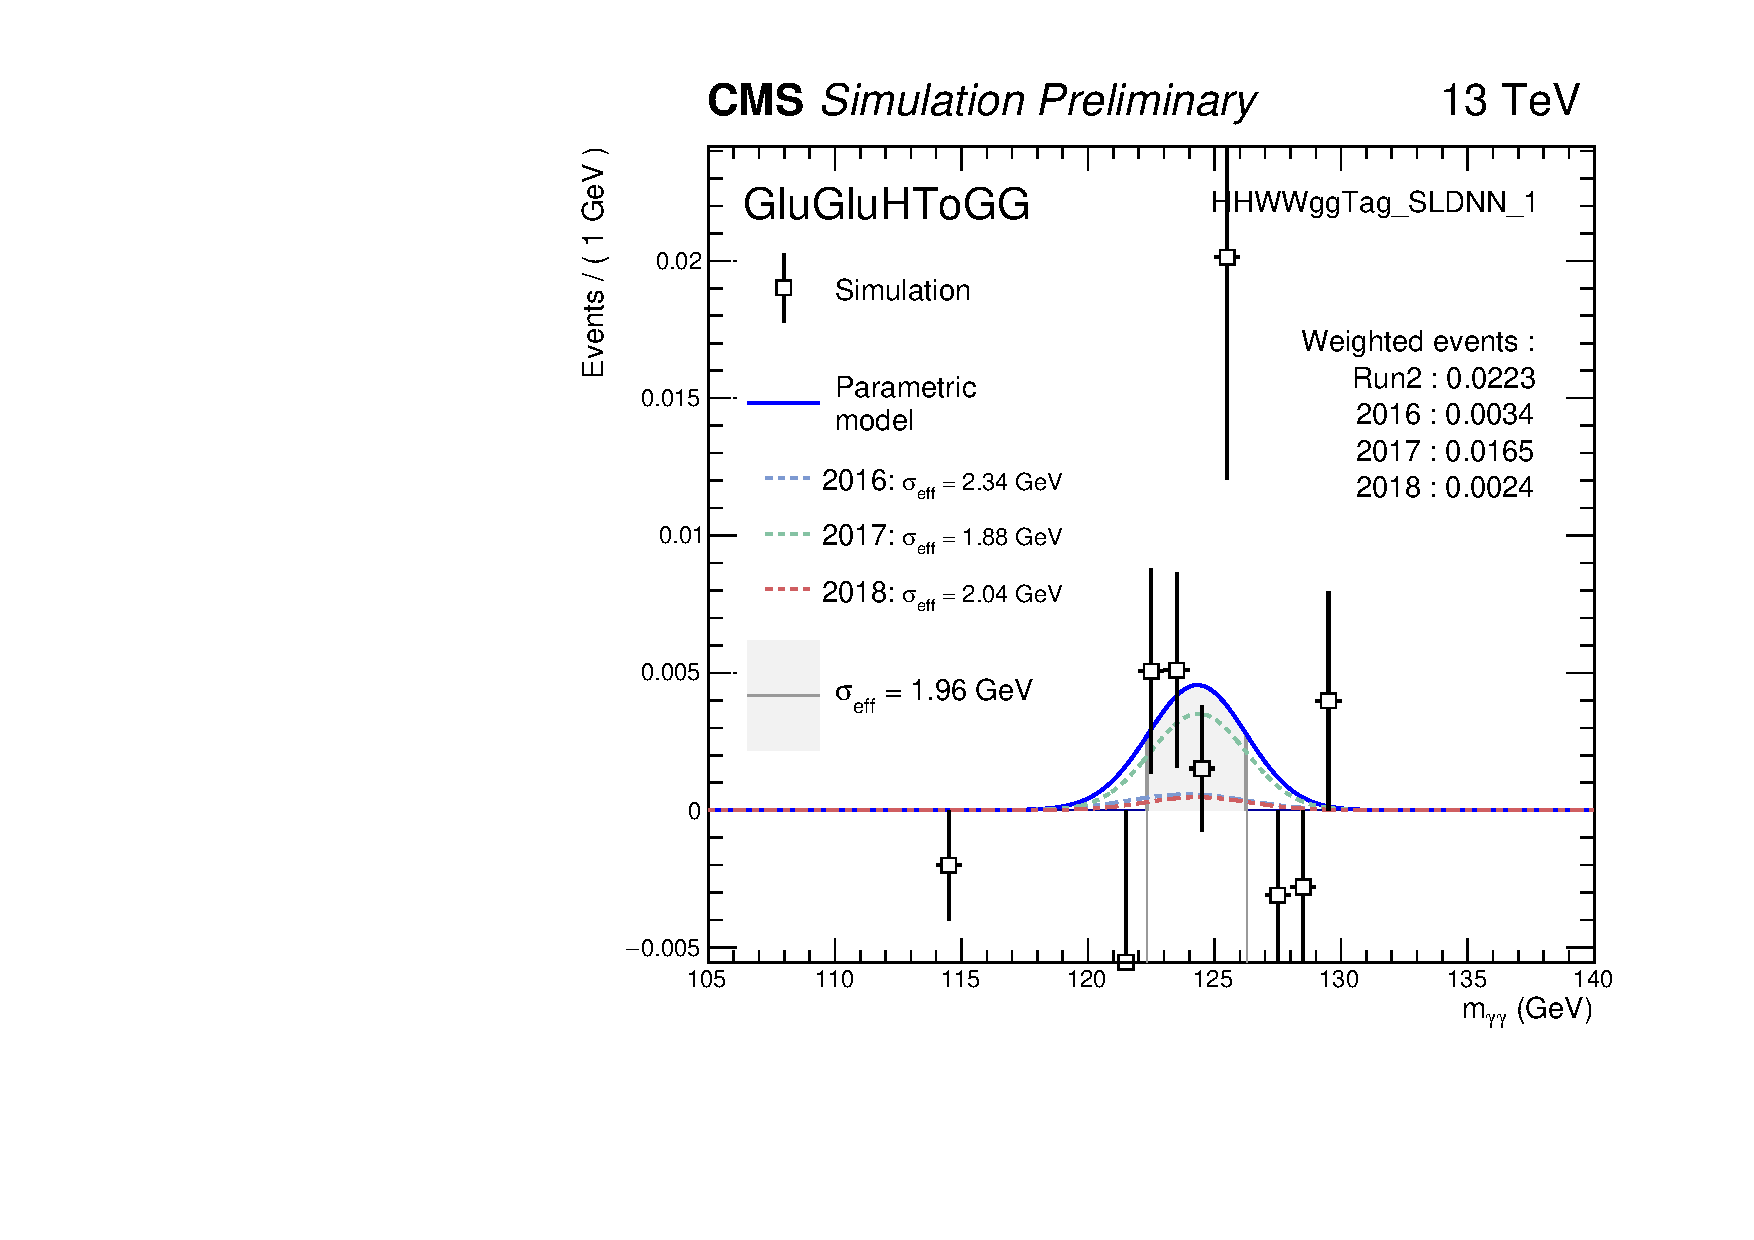
\includegraphics[width=0.45\textwidth]{Sections/HHWWgg/images/AnalyticFitting/SingleHiggs/ggH/SL/smodel_HHWWggTag_SLDNN_1.pdf}}
    \qquad
    \subfloat[VBFHToGG]{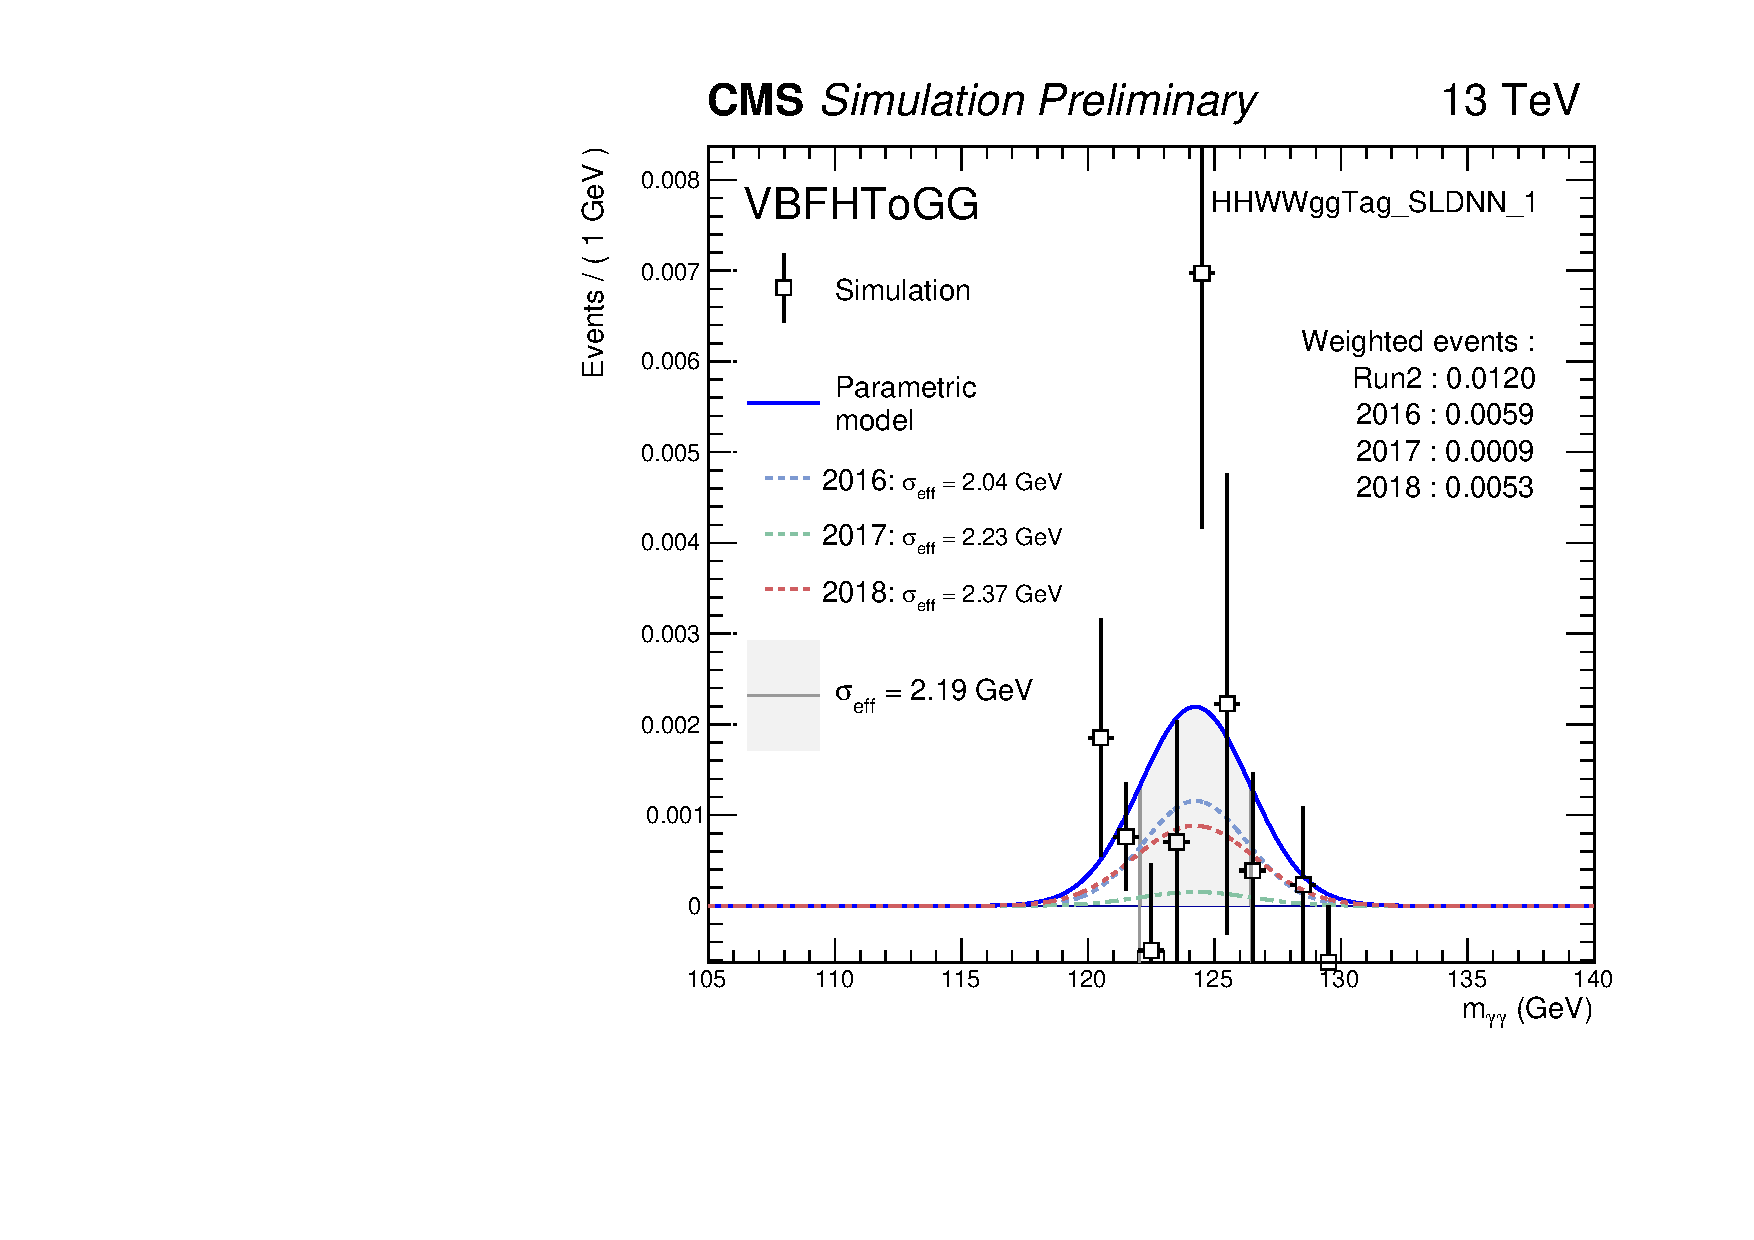
\includegraphics[width=0.45\textwidth]{Sections/HHWWgg/images/AnalyticFitting/SingleHiggs/VBFH/SL/smodel_HHWWggTag_SLDNN_1.pdf}}
    \caption{Semi-Leptonic DNN Category 1 Single Higgs Models}
\end{figure}

\begin{figure}[h!]
    \setcounter{subfigure}{0}
    \centering
    \subfloat[VHToGG]{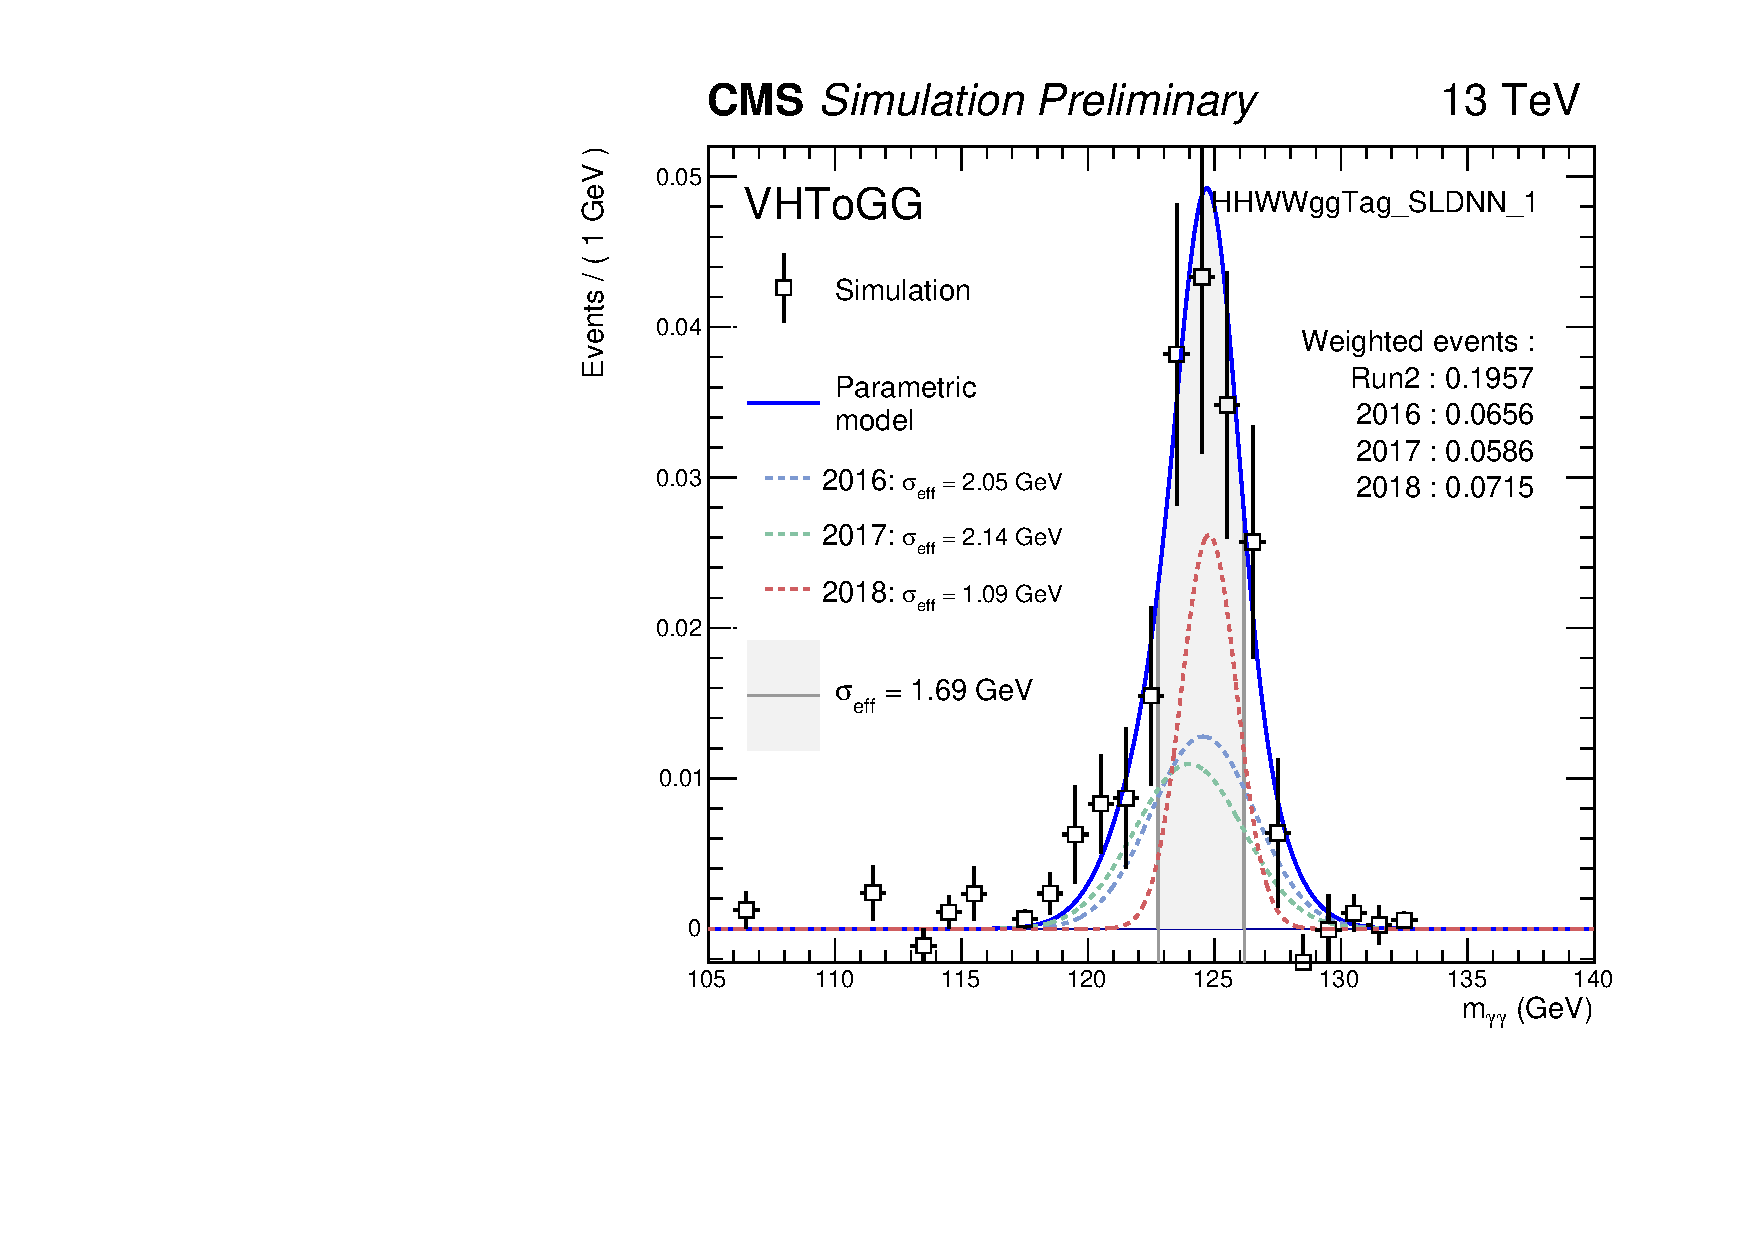
\includegraphics[width=0.45\textwidth]{Sections/HHWWgg/images/AnalyticFitting/SingleHiggs/VH/SL/smodel_HHWWggTag_SLDNN_1.pdf}}
    \qquad
    \subfloat[ttHJetToGG]{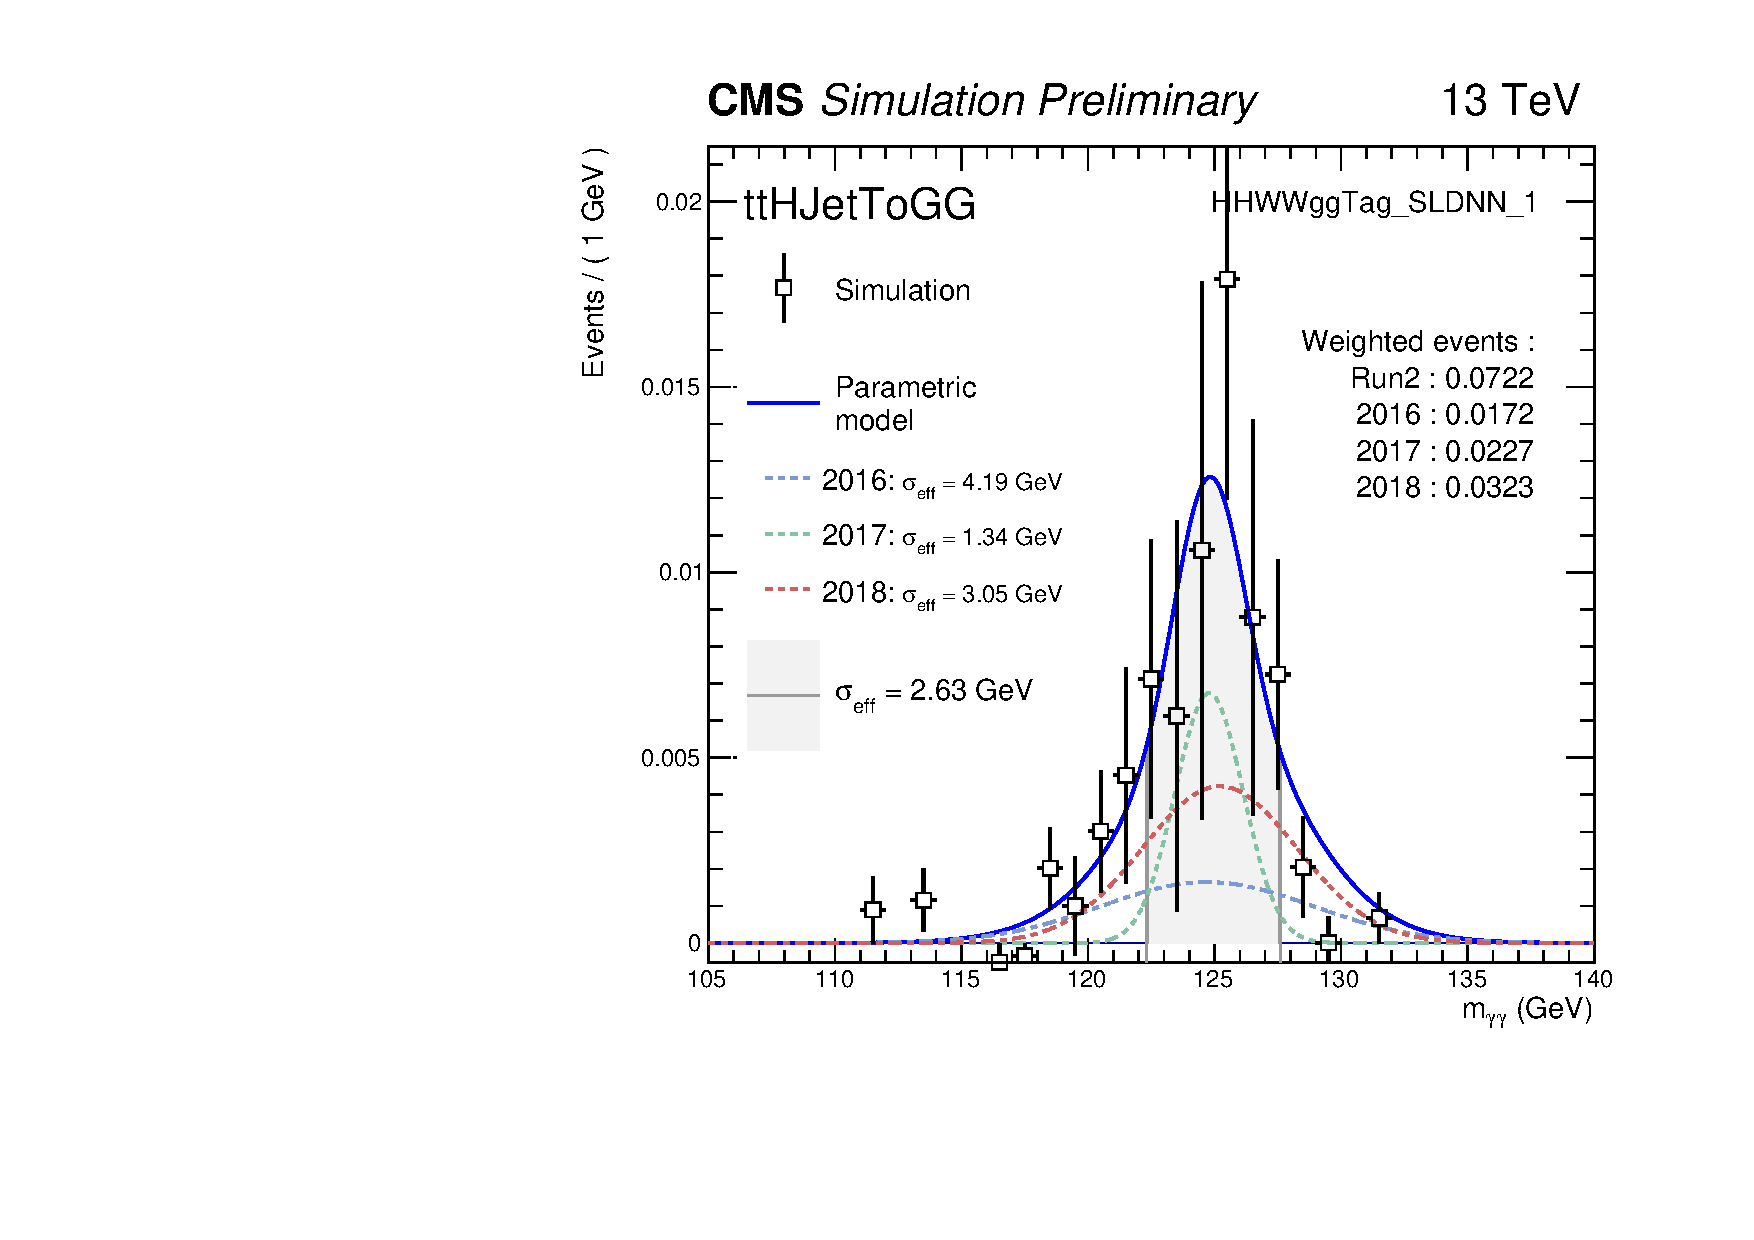
\includegraphics[width=0.45\textwidth]{Sections/HHWWgg/images/AnalyticFitting/SingleHiggs/ttHJet/SL/smodel_HHWWggTag_SLDNN_1.pdf}}
    \caption{Semi-Leptonic DNN Category 1 Single Higgs Models}
\end{figure}

\newpage 

\begin{figure}[h!]
    \setcounter{subfigure}{0}
    \centering
    \subfloat[GluGluHToGG]{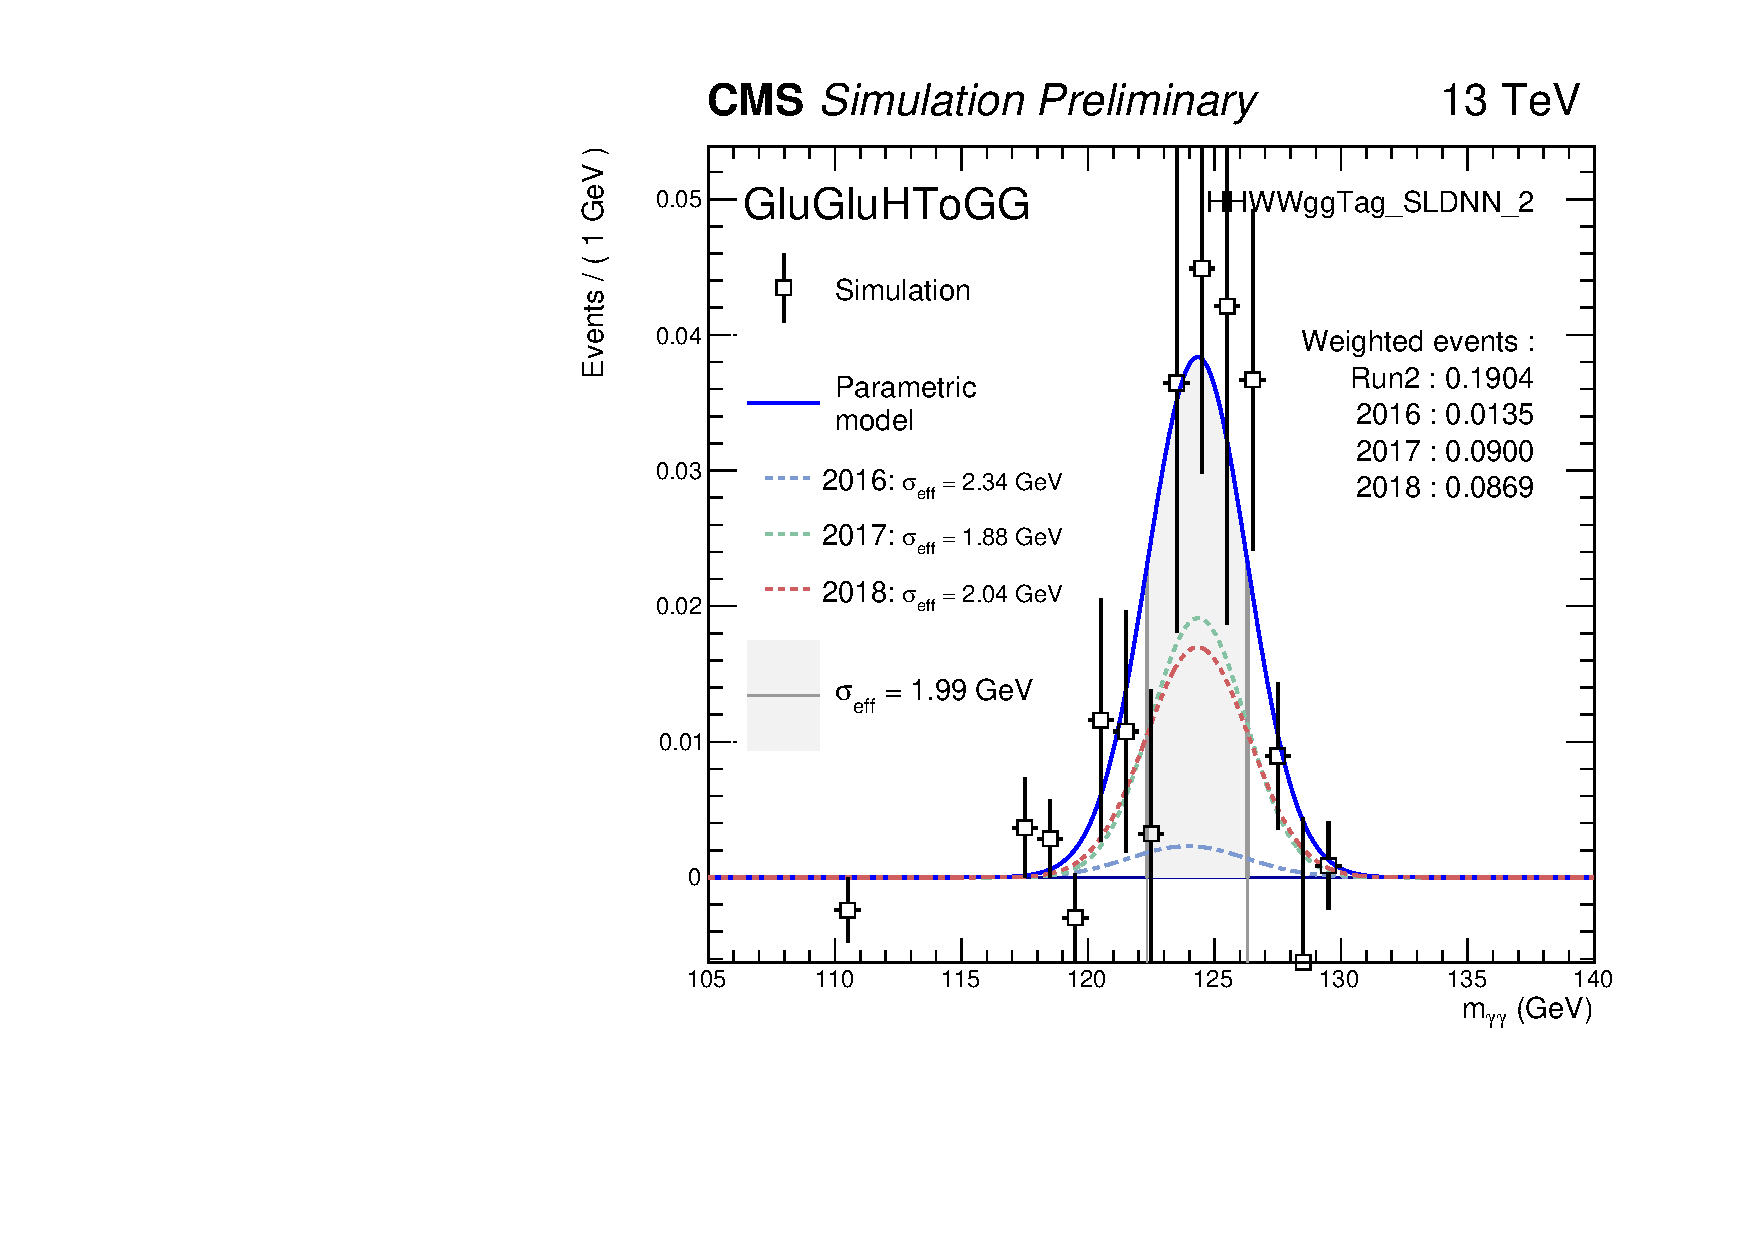
\includegraphics[width=0.45\textwidth]{Sections/HHWWgg/images/AnalyticFitting/SingleHiggs/ggH/SL/smodel_HHWWggTag_SLDNN_2.pdf}}
    \qquad
    \subfloat[VBFHToGG]{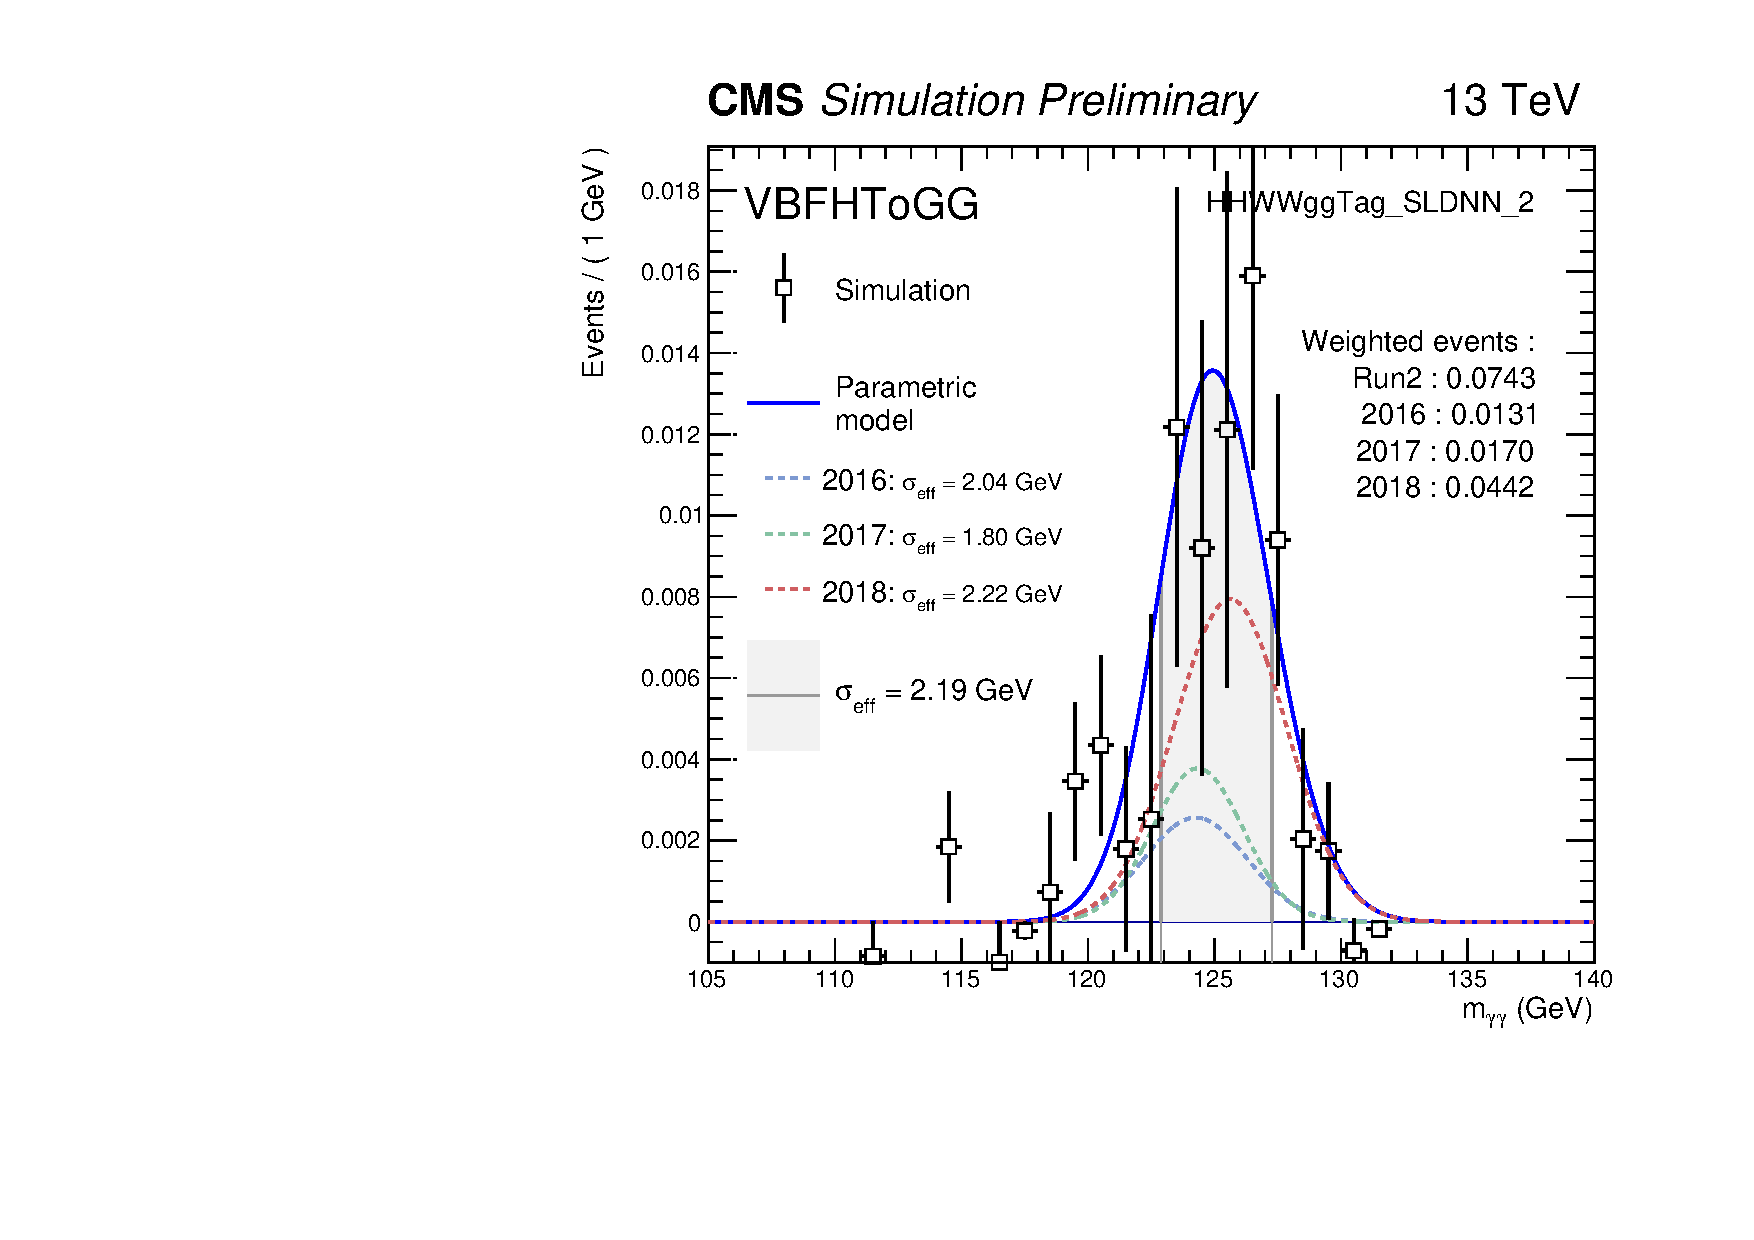
\includegraphics[width=0.45\textwidth]{Sections/HHWWgg/images/AnalyticFitting/SingleHiggs/VBFH/SL/smodel_HHWWggTag_SLDNN_2.pdf}}
    \caption{Semi-Leptonic DNN Category 2 Single Higgs Models}
\end{figure}

\begin{figure}[h!]
    \setcounter{subfigure}{0}
    \centering
    \subfloat[VHToGG]{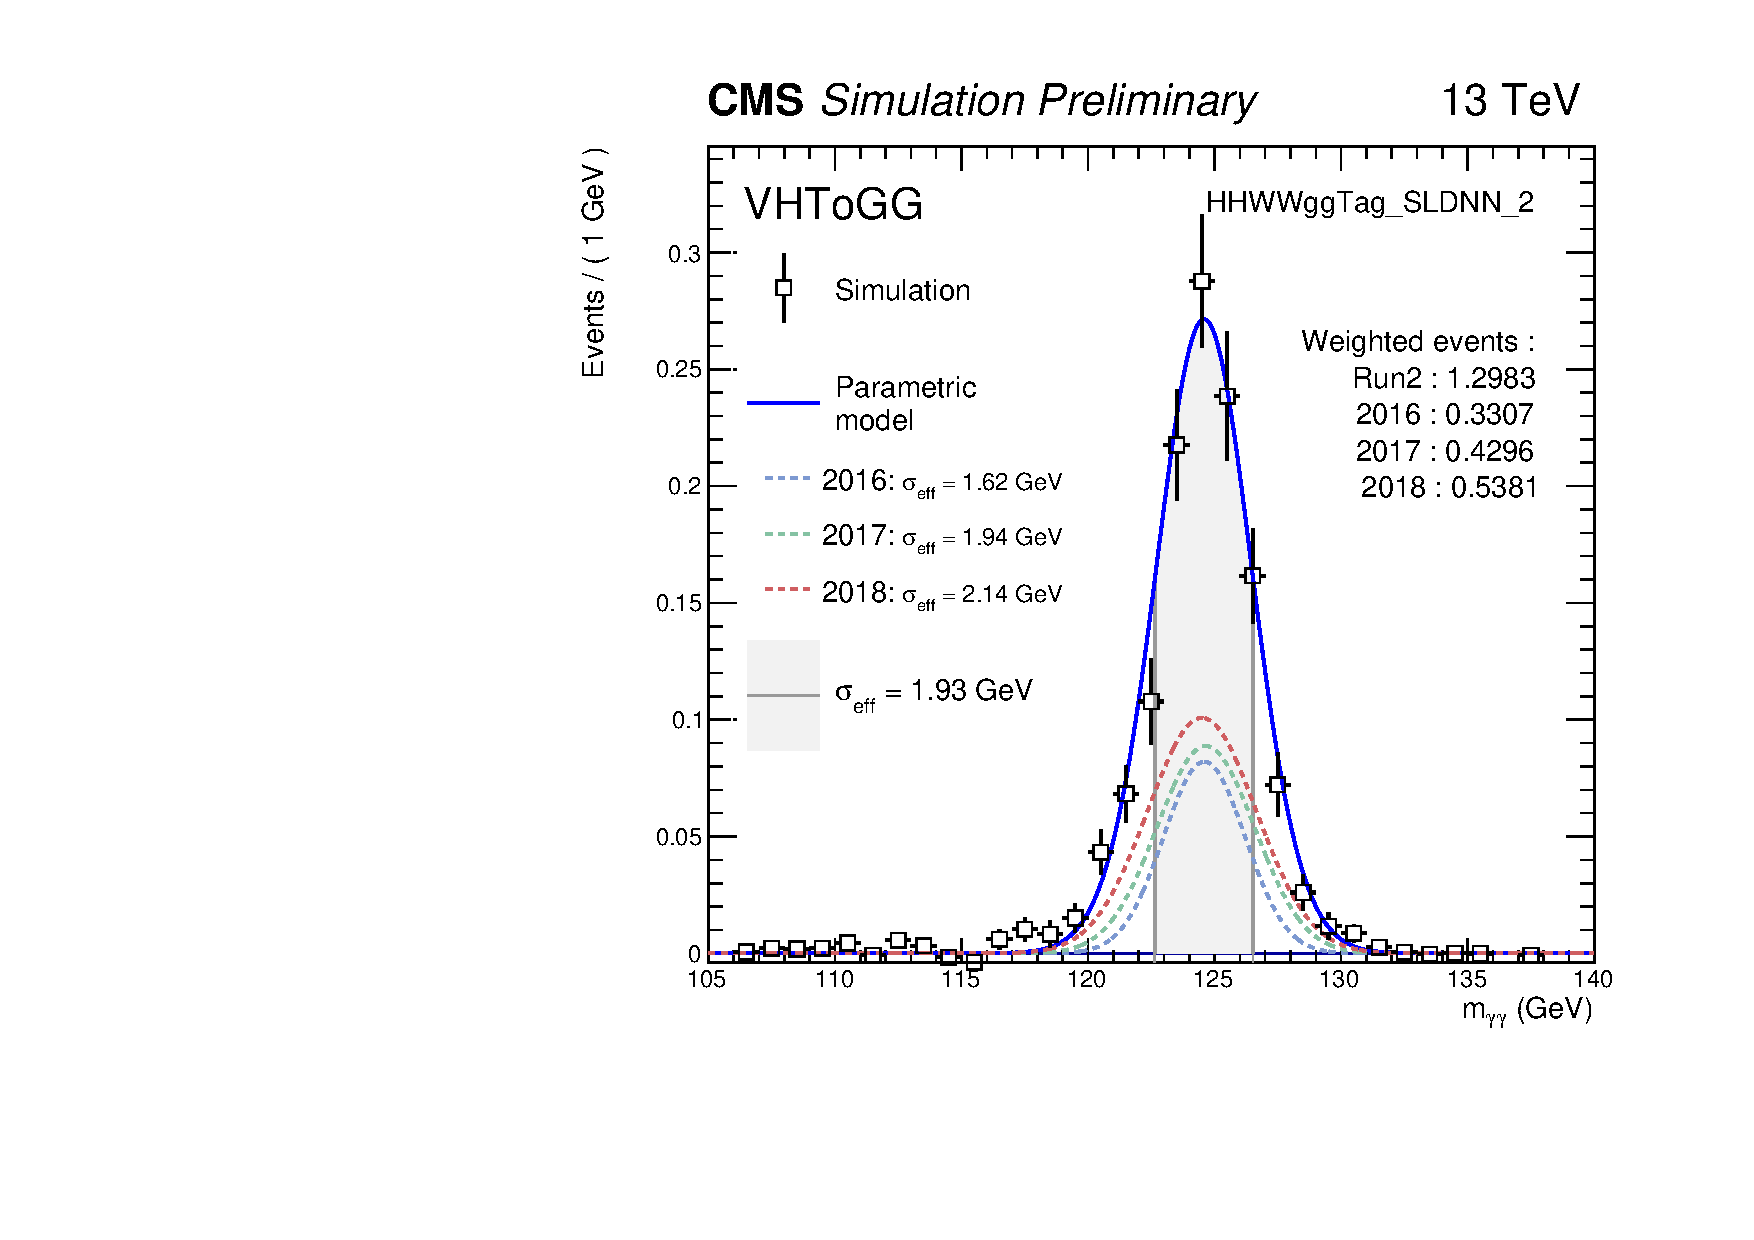
\includegraphics[width=0.45\textwidth]{Sections/HHWWgg/images/AnalyticFitting/SingleHiggs/VH/SL/smodel_HHWWggTag_SLDNN_2.pdf}}
    \qquad
    \subfloat[ttHJetToGG]{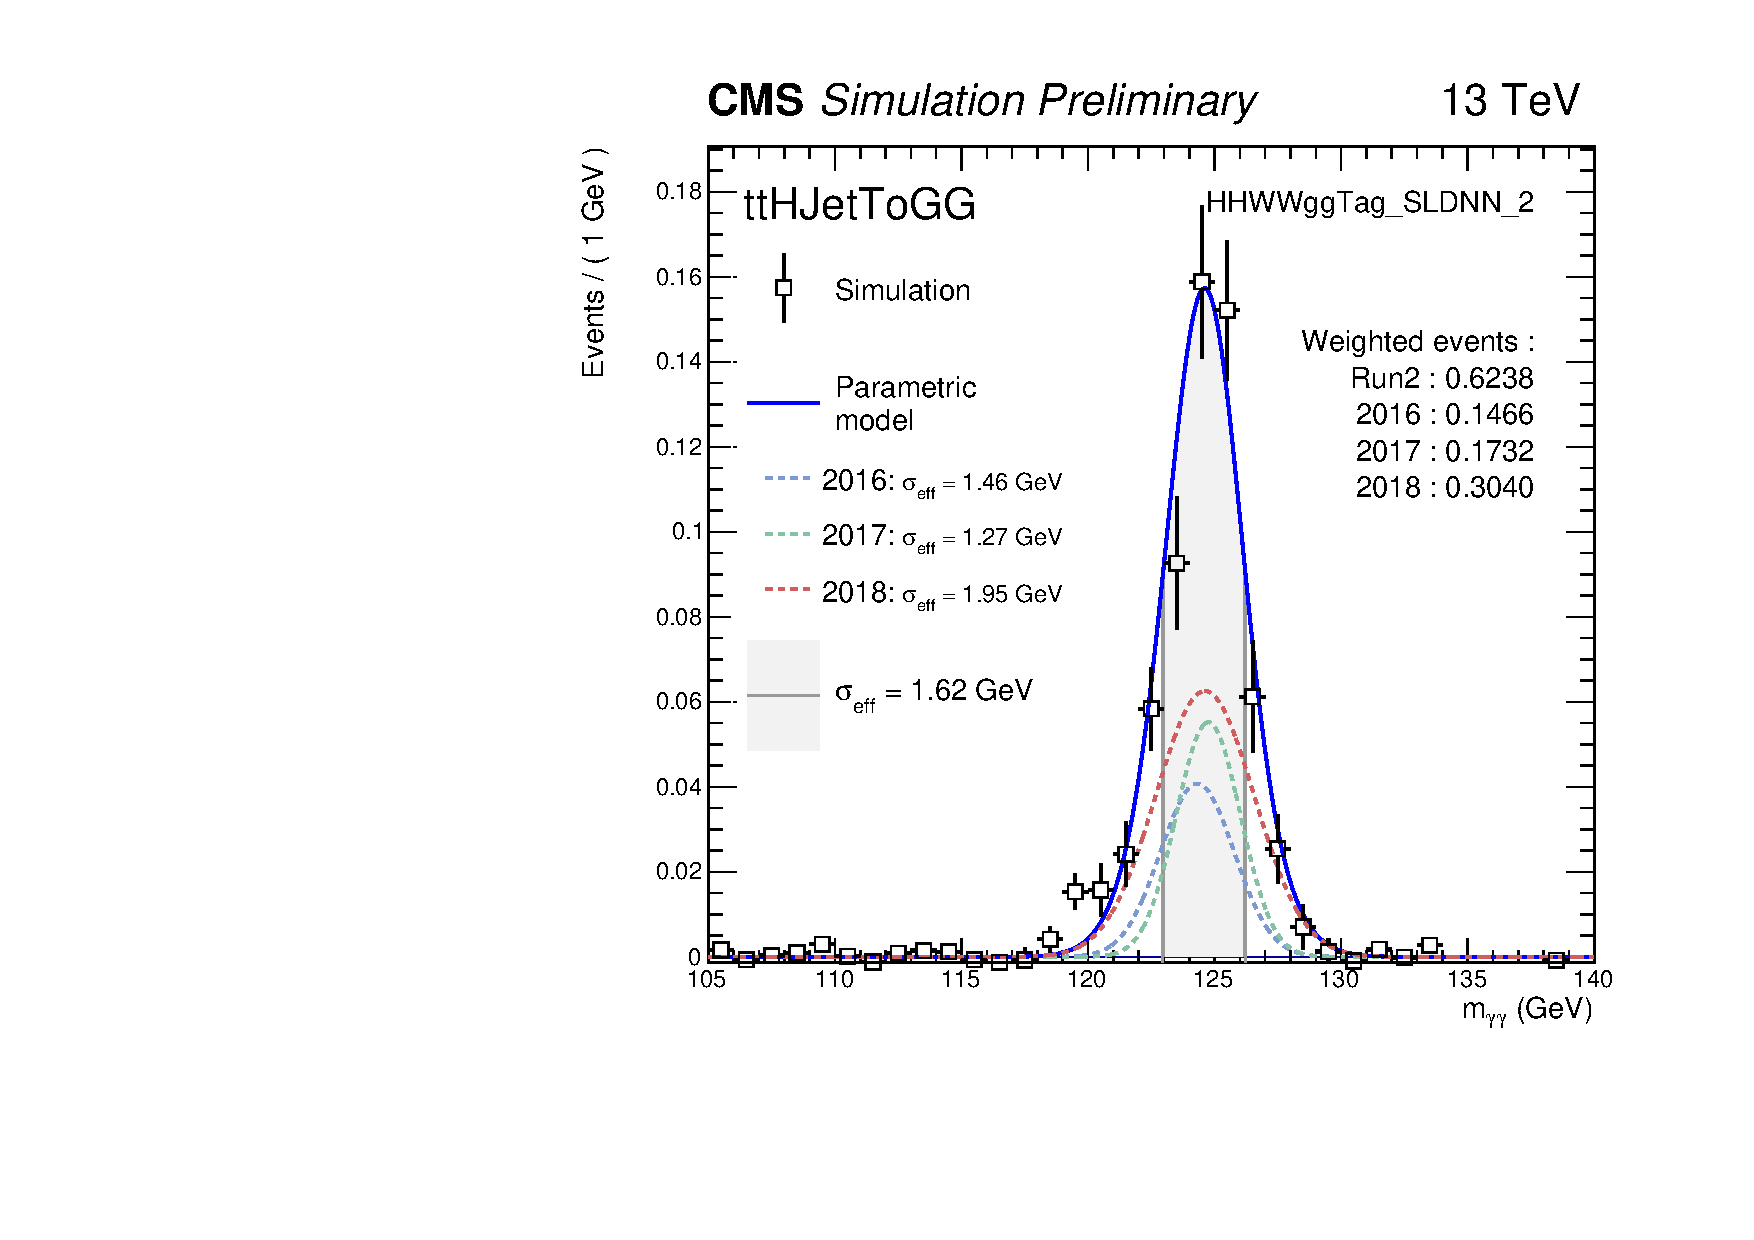
\includegraphics[width=0.45\textwidth]{Sections/HHWWgg/images/AnalyticFitting/SingleHiggs/ttHJet/SL/smodel_HHWWggTag_SLDNN_2.pdf}}
    \caption{Semi-Leptonic DNN Category 2 Single Higgs Models}
\end{figure}

\newpage 

\begin{figure}[h!]
    \setcounter{subfigure}{0}
    \centering
    \subfloat[GluGluHToGG]{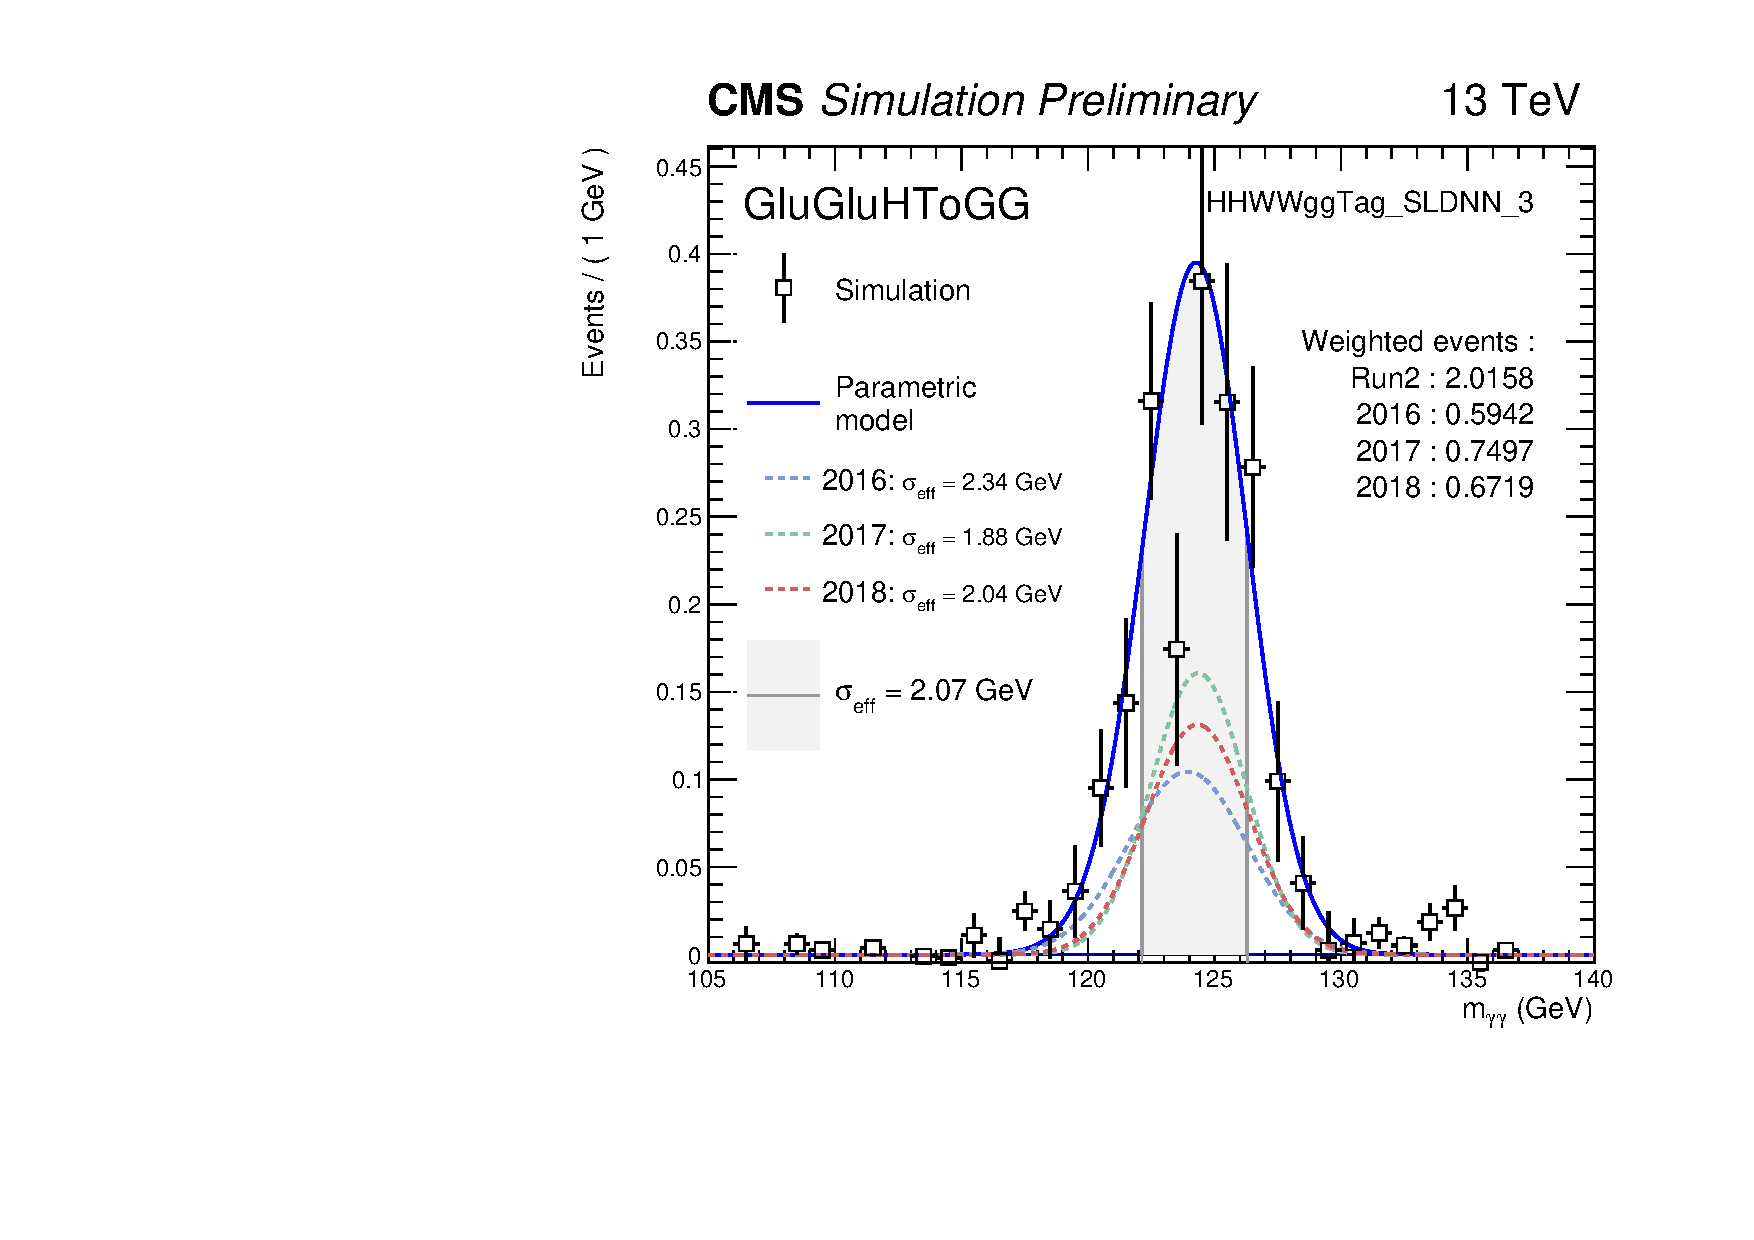
\includegraphics[width=0.45\textwidth]{Sections/HHWWgg/images/AnalyticFitting/SingleHiggs/ggH/SL/smodel_HHWWggTag_SLDNN_3.pdf}}
    \qquad
    \subfloat[VBFHToGG]{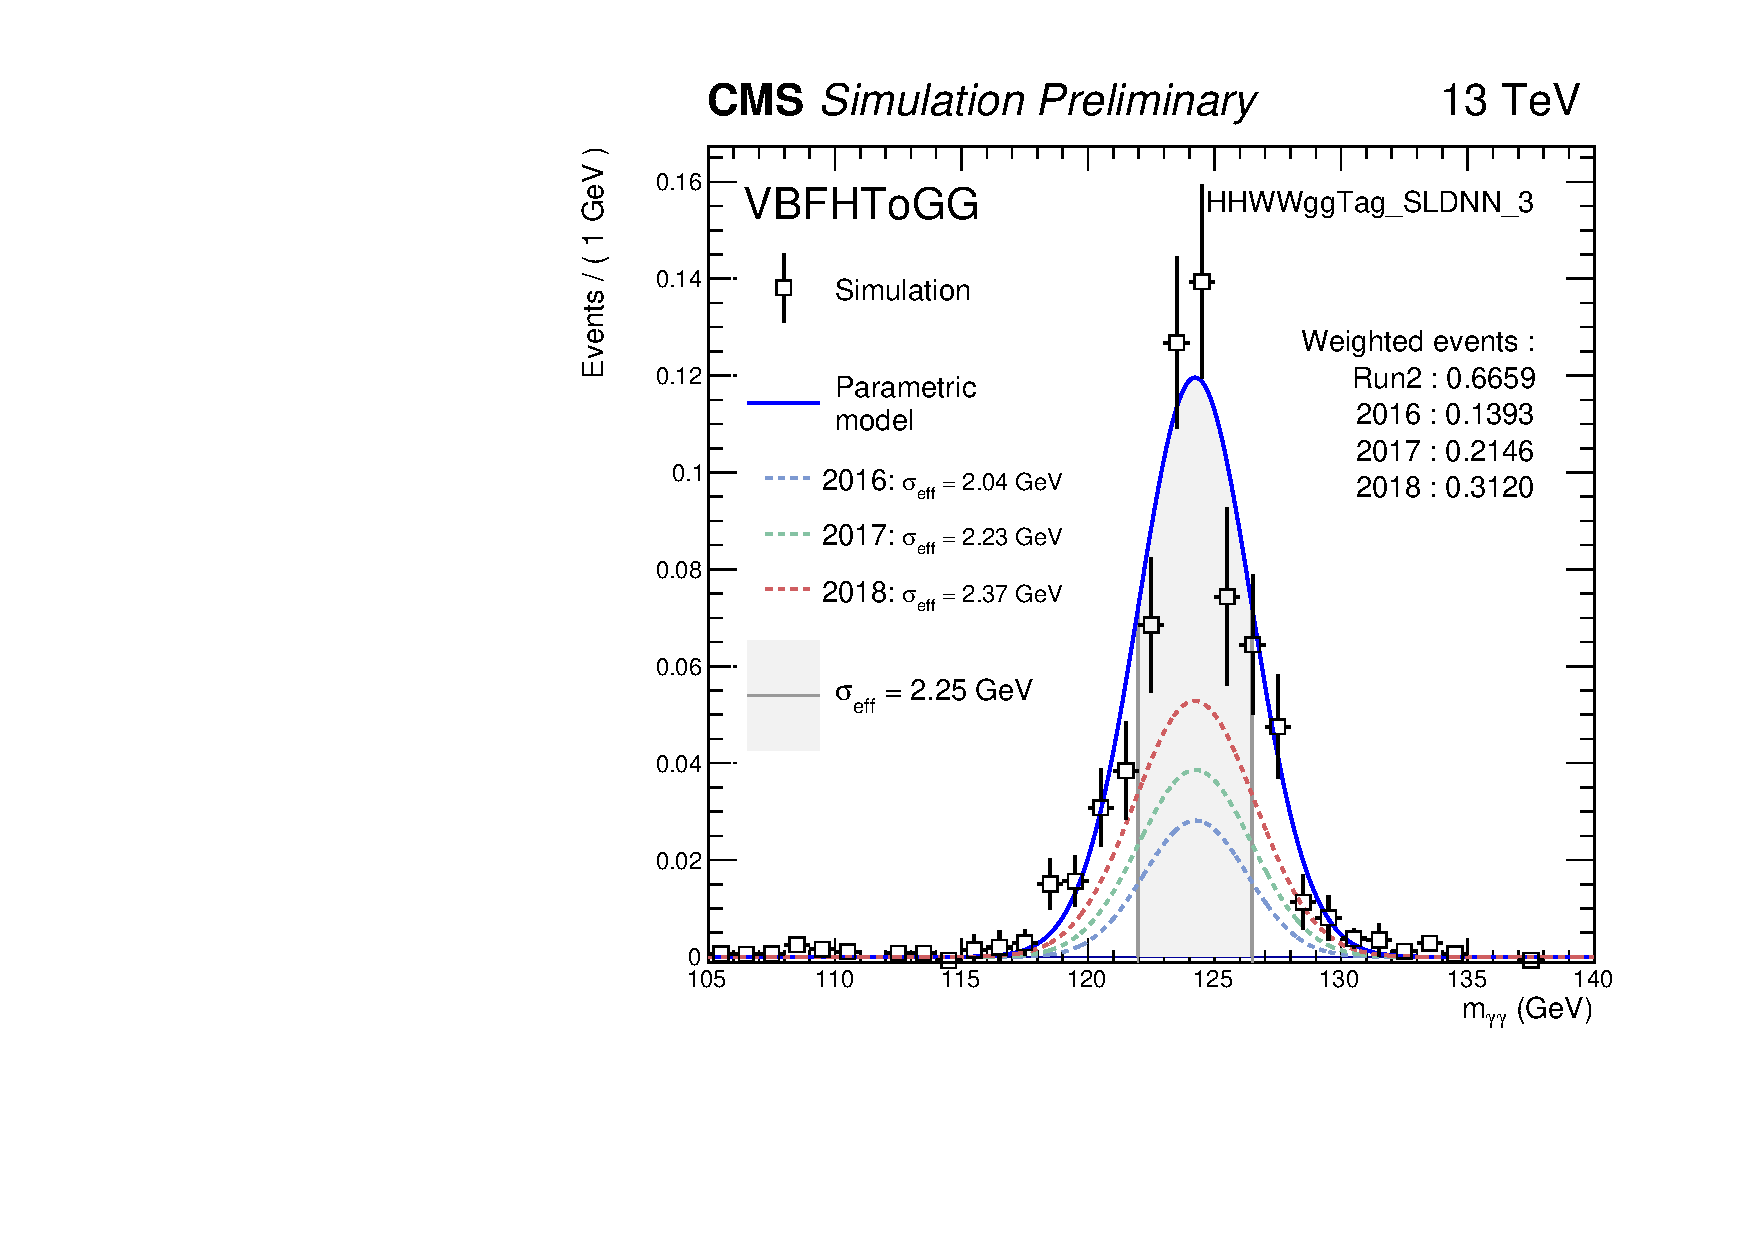
\includegraphics[width=0.45\textwidth]{Sections/HHWWgg/images/AnalyticFitting/SingleHiggs/VBFH/SL/smodel_HHWWggTag_SLDNN_3.pdf}}
    \caption{Semi-Leptonic DNN Category 3 Single Higgs Models}
\end{figure}

\begin{figure}[h!]
    \setcounter{subfigure}{0}
    \centering
    \subfloat[VHToGG]{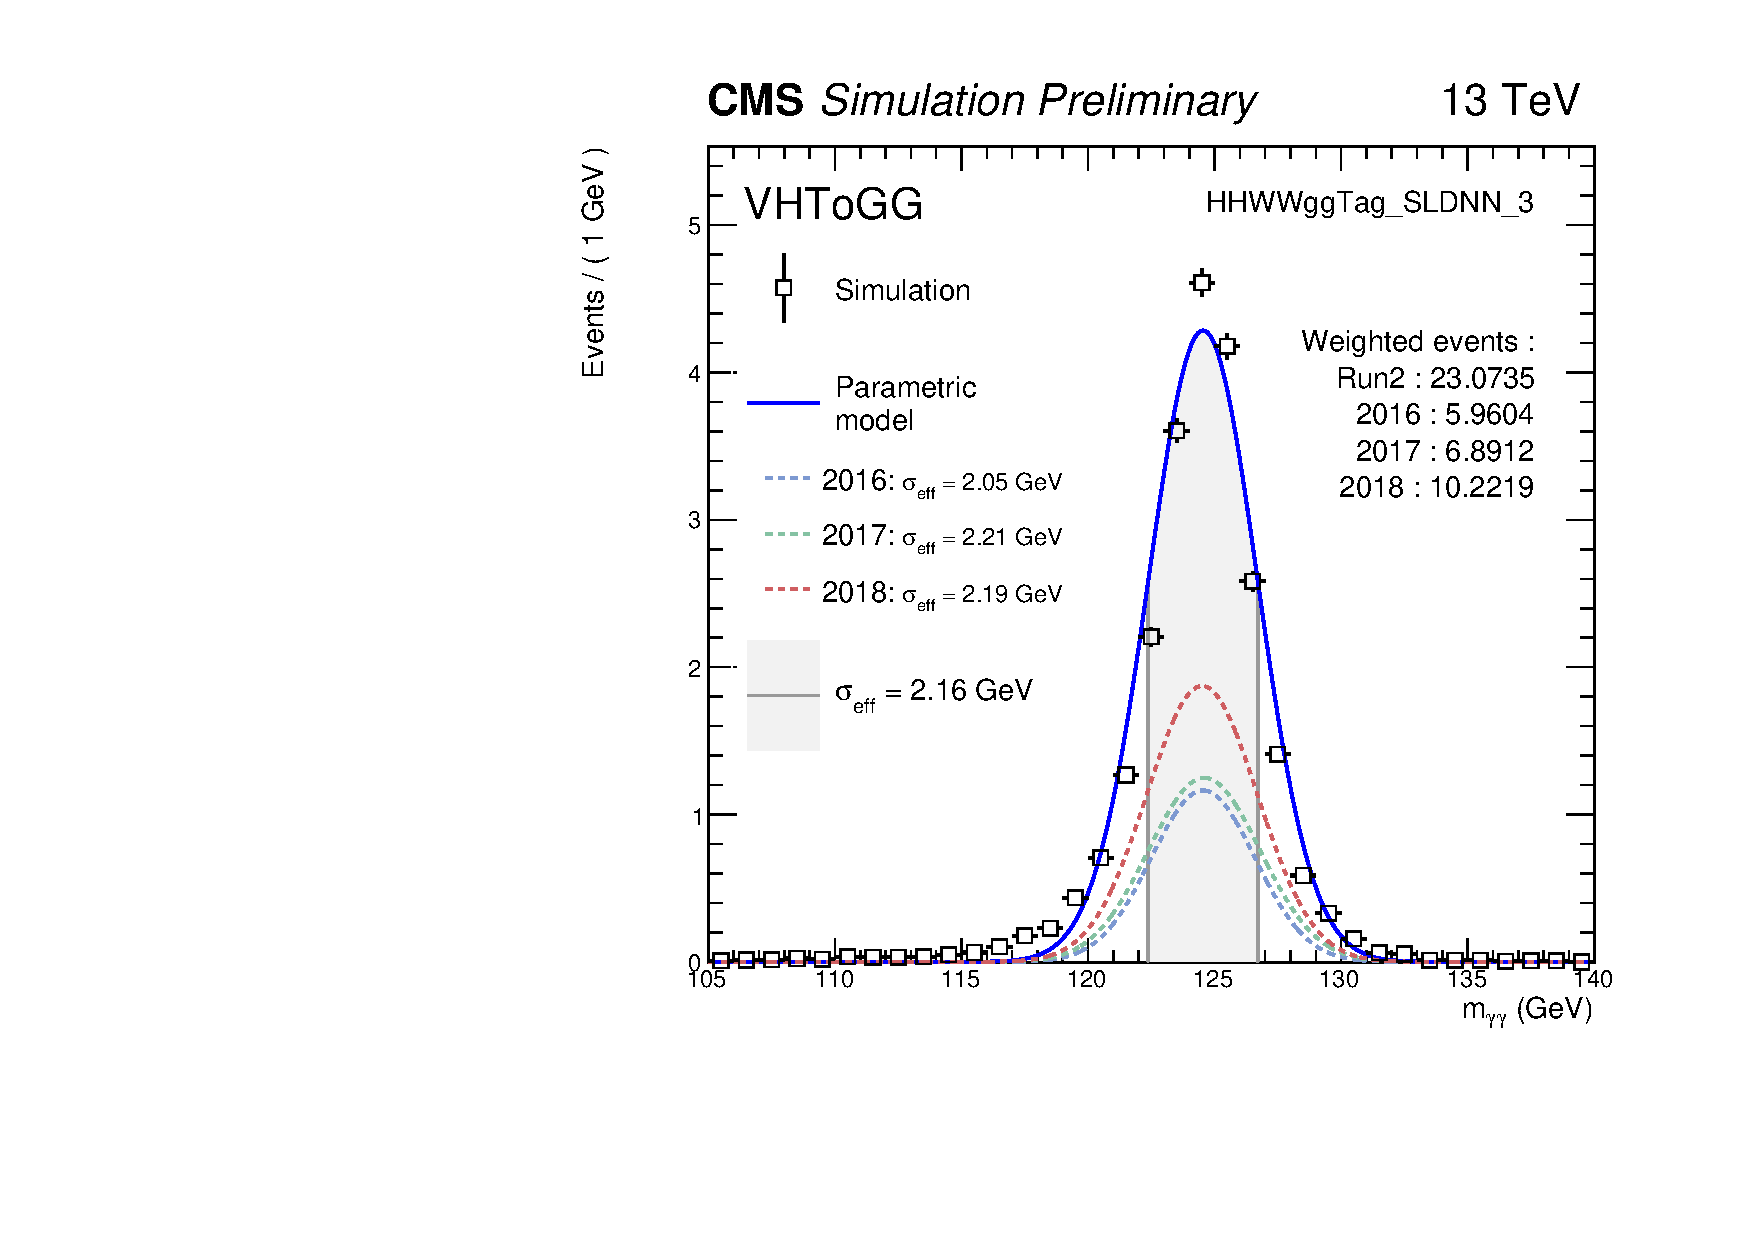
\includegraphics[width=0.45\textwidth]{Sections/HHWWgg/images/AnalyticFitting/SingleHiggs/VH/SL/smodel_HHWWggTag_SLDNN_3.pdf}}
    \qquad
    \subfloat[ttHJetToGG]{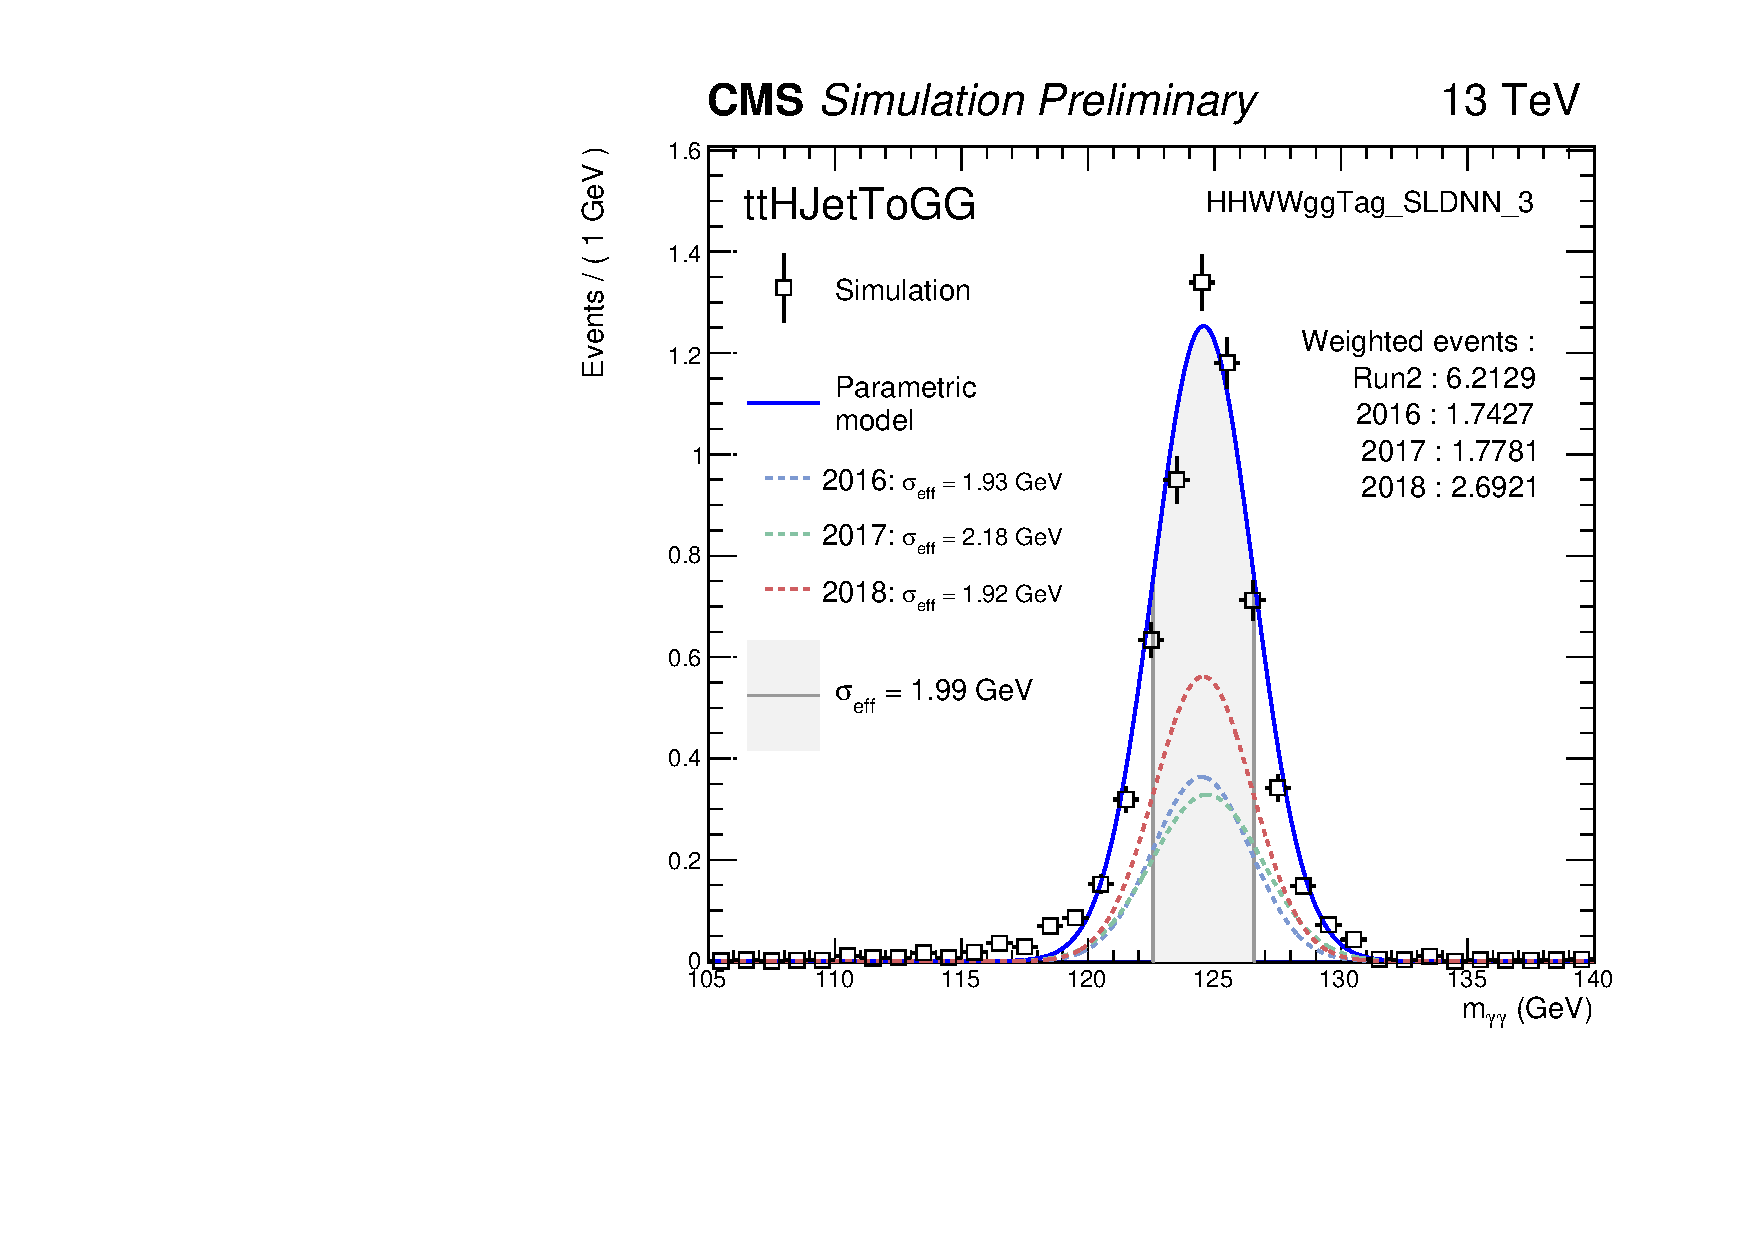
\includegraphics[width=0.45\textwidth]{Sections/HHWWgg/images/AnalyticFitting/SingleHiggs/ttHJet/SL/smodel_HHWWggTag_SLDNN_3.pdf}}
    \caption{Semi-Leptonic DNN Category 3 Single Higgs Models}
\end{figure}